\documentclass[11pt,letterpaper]{article}
\usepackage[T1]{fontenc}
\usepackage{upquote}
\usepackage{microtype}
\DisableLigatures[-]{family=tt*}
\usepackage{mathptmx}
\usepackage[margin=1in]{geometry}
\usepackage{amsmath,amssymb,amsthm}
\usepackage{booktabs,tabularx,longtable,array,multirow}
\usepackage{float}
\usepackage{needspace}
\usepackage{enumitem}
\usepackage{tikz,pgfplots}
\usetikzlibrary{arrows.meta,positioning,fit,calc,shapes.geometric,patterns}
\pgfplotsset{compat=1.17}
\usepackage[font=small,labelfont=bf,textfont=it]{caption}
\usepackage{url,xurl}
\usepackage[hidelinks]{hyperref}
\usepackage{titlesec}
\usepackage{listings}
\usepackage{fancyhdr}
\usepackage{graphicx}
\titleformat{\section}{\normalfont\large\bfseries}{\thesection.}{0.5em}{}
\titleformat{\subsection}{\normalfont\normalsize\bfseries}{\thesubsection}{0.5em}{}
\titleformat{\subsubsection}{\normalfont\normalsize\bfseries}{\thesubsubsection}{0.5em}{}
\setlength{\parindent}{1.5em}
\setlength{\parskip}{2pt}
\renewcommand{\arraystretch}{1.17}
\emergencystretch=3em
\captionsetup{justification=raggedright,singlelinecheck=false}
\lstset{basicstyle=\ttfamily\footnotesize,breaklines=true,breakatwhitespace=true,frame=single,framesep=5pt,showstringspaces=false,columns=fullflexible,aboveskip=8pt,belowskip=9pt}
\setlist{topsep=3pt,itemsep=3pt,parsep=0pt}
\newtheorem{definition}{Definition}
\newcommand{\authorname}{Thor Thor}
\newcommand{\orcidid}{0009-0001-6573-385X}
\tikzset{phase/.style={draw,rounded corners=1.2pt,minimum height=10mm,minimum width=22mm,font=\sffamily\scriptsize,align=center,inner sep=3pt,fill=white},observed/.style={phase,line width=0.85pt},unseen/.style={phase,dashed},arr/.style={-{Stealth[length=2.2mm]},semithick},darr/.style={-{Stealth[length=2.2mm]},dashed,semithick},tbl/.style={font=\sffamily\tiny}}
\hypersetup{pdftitle={Firmware-Update Observability in a Single-Earbud AirPods 4 ANC Configuration},pdfauthor={Thor Thor},pdfsubject={Open-source empirical study of macOS UARP updater logs, bounded direct-transport diagnostics, and a missing companion AirPod},pdfkeywords={AirPods 4 ANC, A3056, UARP, firmware update, macOS, MobileAsset, Bluetooth, L2CAP, single-earbud, repairability, reproducibility}}
\begin{document}
\begin{center}
{\LARGE\bfseries Firmware-Update Observability in a Single-Earbud AirPods 4 ANC Configuration\par}
\vspace{0.65em}
{\large A macOS UARP Case Study of Asset Discovery, Update Initiation, Device-State Verification, and Bounded Direct-Transport Diagnostics\par}
\vspace{1.1em}
{\large \authorname\par}
\vspace{0.25em}
{\small Independent Open-Source Researcher, THOR-SEC / Project THOR | ECHO TRACE\\
ORCID: \href{https://orcid.org/\orcidid}{\orcidid} \quad \url{codethor@gmail.com}\\
GitHub: \url{https://github.com/codethor0} \quad \url{https://codethor0.github.io/thor-sec/}\par}
\vspace{0.35em}
{\small Conducted independently on the author's own time. Not sponsored by, affiliated with, or representative of any employer.\par}
\vspace{0.35em}
{\small Research observation dates: November 6--7, 2026.\par}
\vspace{0.8em}
{\centering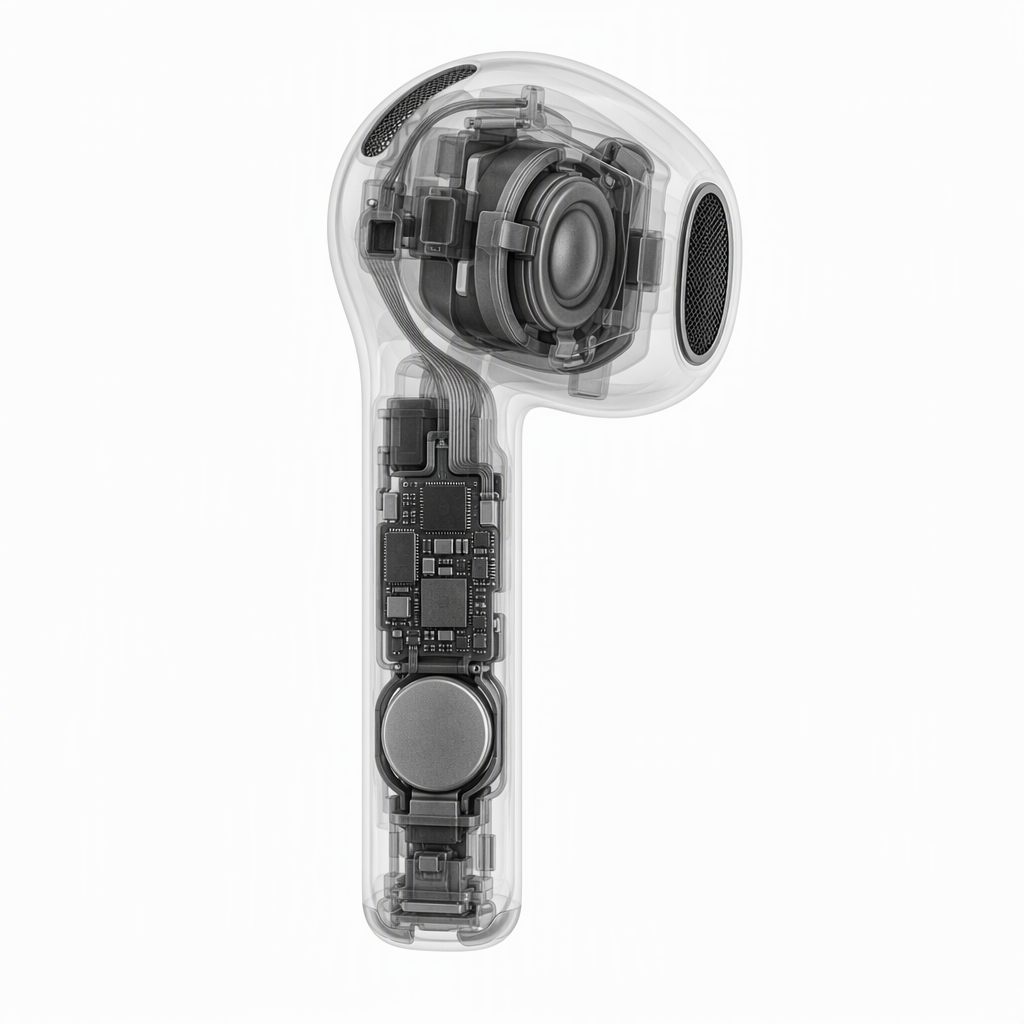
\includegraphics[width=0.34\linewidth]{figures/earbud_xray_bw.png}\par}
\vspace{0.3em}
{\footnotesize\itshape AI-generated conceptual cutaway of an open-ear wireless earbud;\\not a radiograph, device scan, or verified A3056 internal layout.\par}
\end{center}
\vspace{0.5em}
\begin{abstract}
Wireless earbuds operate on embedded firmware, yet their update process is largely automatic and offers limited user-visible diagnostics. This paper reports an independent macOS investigation of an AirPods 4 with Active Noise Cancellation (ANC) configuration in which the right earbud was lost and only the left A3056 remained. The target, Bluetooth product identifier \texttt{0x201B}, reported firmware \texttt{8B21}; Apple's published release and the macOS A3056 catalog listed \texttt{9A348}. The host contained a corresponding Universal Accessory Restore Protocol (UARP) firmware payload and logged updater registration of the remaining earbud and case at \texttt{8.1.21.0}. I reconstructed firmware and Bluetooth state, separated a distinct non-ANC AirPods device, evaluated 60 ANC host-state samples under three intervention conditions, and triaged 3,257 updater log records. An initial controlled trial stopped during a locally imposed connected-audio preflight while the earbud was in its charging case. A subsequent manual intervention completed an \texttt{airpods-fw} dry run and posted a system-wide Apple update-scan notification; the preserved transcript did not record the scan timestamp, so the duration of the case-closed interval cannot be reconstructed. Two subsequent cached checks reported \texttt{8B21}. At 16:49:43 CST on November 7, 2026, \texttt{airpods-fw} reported the target connected and on \texttt{8B21}; a separate macOS Bluetooth inventory likewise showed the connected \texttt{0x201B} target and case on \texttt{8B21}. The bounded trial therefore produced no observed firmware-version change, with the dwell time unauditable. A follow-on series of bounded direct-transport experiments (F-05 through F-13), information-only in most runs with three explicitly authorized offer sessions as exceptions, then established device identity over GATT, confirmed the UARP service, and attempted Apple Accessory Protocol (AAP) and UARP information queries from a native macOS host. From a paired-but-disconnected state at case-lid open, a single L2CAP control channel opened, the AAP handshake was acknowledged, and UARP sync and version-request frames were transmitted, but no valid UARP version reply was received before the accessory closed the channel. In three separate bounded sessions on the same channel, the accessory itself confirmed running firmware \texttt{8.1.21.0} and a staged firmware of \texttt{0.0.0.0}, acknowledged a single firmware offer referencing the cached \texttt{9A348} build in each session, and then produced client-decoded terminal processing responses before any image-data request. The F-08U/V flags \texttt{0x0003} admit more than one interpretation under the cited reverse-engineering notes. No image bytes were served and no staging or Apply command was sent. From a connected audio state, the same control channel was repeatedly unavailable. The inspected evidence did not identify an A3056-specific eligibility decision or a confirmed firmware transfer or activation; the significance and cause of the observed terminal offer-processing notifications, including any eligibility decision, remain unresolved. The missing companion earbud remains a testable dependency hypothesis, and third-party analysis of a sibling product indicates that case-mediated update completion requires both buds while host-driven staging does not. The study provides a dated, reproducible account of firmware availability, scan initiation, connected-device verification, direct-transport behavior, and the diagnostic evidence needed to resolve this maintenance edge case.
\end{abstract}
\vspace{-0.3em}
\noindent\textbf{Keywords:} AirPods 4 ANC; A3056; single-earbud maintenance; firmware update; UARP; macOS; MobileAsset; reproducibility; Bluetooth; L2CAP; repairability
\medskip

\section{Introduction}\label{sec:introduction}
Modern wireless earbuds are embedded computing devices. Their visible features include playback, microphones, environmental noise control, and connection management; their implementation also depends on firmware resident in the accessory. A user may experience the device as ordinary audio hardware while its maintenance process follows software release, discovery, staging, transfer, and activation rules that are largely hidden from the user interface. Apple's public instructions describe automatic updates while AirPods are in a closed, powered charging case within range of a network-connected Apple host \cite{applefw}. A separate manual firmware-image selection option is not described in those instructions.

This investigation began with a practical failure mode: one AirPods 4 ANC earbud remained after the right earbud was lost. The remaining left unit was operational as a Bluetooth audio accessory, but continued to report firmware \texttt{8B21}. The publicly listed release for its model family was \texttt{9A348}. Before the study, I had left the earbud charging for extended periods without observing an update. I also noticed changes in noise-control settings and ear discomfort during use. Those observations prompted a forensic examination of the update path rather than a claim about the source of the symptoms.

An important consumer maintenance question follows. If a user loses one earbud but still has a functioning partner and charging case, does the remaining unit continue to receive firmware updates? A negative outcome could arise at several different points: no suitable image, inability to discover the accessory, update-policy eligibility, unavailable companion device, case or lid state, transport failure, or a host-side version record that was not refreshed. A single unchanging version number cannot distinguish these possibilities.

\paragraph{Research objective.} This paper reconstructs the observed state transitions for one device and identifies which stages of firmware delivery were visible to macOS. It records the aborted preflight and the subsequent manual scan request, then compares connected-device firmware state before and after the case-closed interval. It then bounds the question further with a series of bounded direct-transport experiments: information-only diagnostics in most runs, plus three explicitly authorized sessions (F-08T, F-08U, F-08V) that each transmitted one firmware offer referencing the cached candidate image. No firmware image was ever transferred, staged, or applied in any run. The work is a single-case empirical study, with data and reproducibility aids selected for public review.

\paragraph{Contributions.} The case contributes (1) a model-specific record separating AirPods 4 ANC from a different AirPods 4 device paired with the same Mac; (2) dated evidence of an old installed version alongside a locally cached newer UARP asset; (3) reconstruction of firmware asset-manager and endpoint-registration messages; (4) an ANC host-state intervention series that distinguishes a third-party control request from later native-interface state; (5) quantified triage of updater log noise; (6) a completed, case-closed scan experiment with a connected-device outcome and an explicit success criterion; and (7) a bounded direct-transport diagnostic series establishing that the accessory accepts a single host L2CAP control-channel open from a paired-but-disconnected state, acknowledges an AAP handshake, answers device-side UARP information queries with its own running (\texttt{8.1.21.0}) and staged (\texttt{0.0.0.0}) firmware records, acknowledges an offer referencing the cached \texttt{9A348} build and then emits client-decoded terminal processing notifications before requesting any image data, while the same channel is unavailable from a connected audio state; and (8) read-only structural analysis of the cached \texttt{9A348} payload, in which all 17 declared payloads parsed as bounds-valid and the 6.8\,MB FTAB payload passed a SHA-256 integrity check. These are method contributions and case findings, not a generalization to every AirPods configuration.

\section{Background, Related Work, and Evidence Model}\label{sec:background}
\subsection{Firmware and the charging-case update process}
Apple publishes firmware versions separately for different AirPods families and provides a standard update process using a paired iPhone, iPad, or Mac, Wi-Fi, Bluetooth proximity, a powered charging case, and a closed lid \cite{applefw}. The procedure places the earbuds in the powered case, closes the lid, keeps the case near the host, and waits at least 30 minutes; charge state is a prerequisite, and Apple's charging guidance covers the case-power requirement \cite{applecharge}. At the time of this investigation, Apple's AirPods 4 ANC entry listed release \texttt{9A348}. Its corresponding release notes described a Custom EQ feature for eligible products; earlier builds also carried general improvements. The existence of a version difference establishes an observable maintenance gap without identifying the contents of every intermediate release.

For users without a network-connected Apple host nearby, the same support document describes setting up an appointment at an Apple Store or an Apple Authorized Service Provider to update the firmware. That is a vendor-documented service update path; it does not, by itself, establish whether the service path accepts a single surviving earbud, and it does not provide a user-selectable firmware image. Apple's repair program documentation is the corresponding service channel reference \cite{applehelp}.

For me, the firmware question was practical. The remaining earbud could still connect to my Mac. The unknown is whether its update eligibility is evaluated as an individual accessory, a two-earbud set, a case-linked group, or a combination. Public update instructions use the plural \emph{AirPods} but do not define the single-surviving-earbud edge case. That omission makes empirical verification and vendor clarification useful.

\subsection{Related work}
Three bodies of prior work bound this study. First, the open-source \texttt{airpods-fw} utility \cite{airpodsfw} can inspect known device firmware, retrieve Apple release and catalog metadata, inspect local asset records, request an accessory scan, and observe macOS updater logs. Its authors explicitly state that the project has not performed or verified an actual firmware installation; it is an observability tool, not a flasher. Second, the Calvados project published a static analysis of AirPods Pro 2 (USB-C) firmware build \texttt{9A348} and a reported successful update of that model from \texttt{7.1.21} to \texttt{9.0.348} performed from a non-Apple (Linux) host over the buds' GATT UARP service, together with an analysis of the case-mediated sibling-update state machine \cite{calvados}. Third, the LibrePods project hosts the community discussion of that update, including the before/after device-reported version strings and a reported community bricking incident during a non-Apple update attempt with no Apple recovery path \cite{librepods612}.

Two Calvados findings are directly relevant to the missing-companion question, with an explicit hardware boundary. On AirPods Pro 2 (USB-C), the buds' firmware payload carries an Apple-signed manifest binding no device-specific ECID and no nonce, so bud installation does not require a live Apple signing exchange; and the charging case's copy-and-apply logic reads both buds' version records only when both buds are present, while host-driven staging targets the primary bud alone. Every one of those claims is scoped by its authors to AirPods Pro 2 (USB-C), a different product family from the A3056 target of this study. The shared H2 generation and the shared \texttt{9A348} train make architectural similarity plausible, but plausible is not established: offer filters, transport tables, and case state machines can differ per model. This study therefore treats the Calvados results as the closest adjacent evidence, cites them wherever they sharpen a hypothesis, and does not transfer them to A3056.

\subsection{Evidence stages: from a catalog entry to a confirmed version}
I distinguish a firmware update's observable stages rather than treating an available asset as installed software. Figure~\ref{fig:pipeline} summarizes the evidence boundary.

\begin{figure}[htbp]\centering
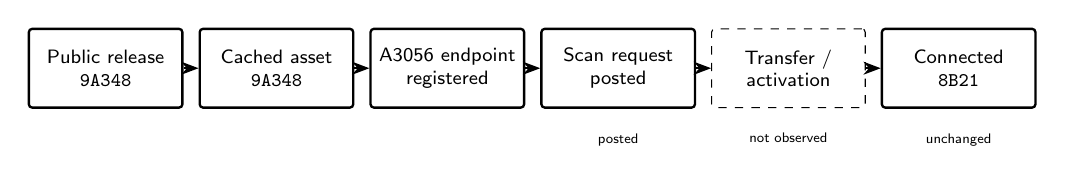
\begin{tikzpicture}[node distance=0.19cm]
\node[observed,minimum width=1.95cm] (a) {Public release\\\texttt{9A348}};
\node[observed,minimum width=1.95cm,right=of a] (b) {Cached asset\\\texttt{9A348}};
\node[observed,minimum width=1.95cm,right=of b] (c) {A3056 endpoint\\registered};
\node[observed,minimum width=1.95cm,right=of c] (d) {Scan request\\posted};
\node[unseen,minimum width=1.95cm,right=of d] (e) {Transfer /\\activation};
\node[observed,minimum width=1.95cm,right=of e] (f) {Connected\\\texttt{8B21}};
\draw[arr] (a) -- (b);\draw[arr] (b) -- (c);\draw[arr] (c) -- (d);
\draw[darr] (d) -- (e);\draw[darr] (e) -- (f);
\node[font=\sffamily\tiny,below=0.19cm of d] {posted};
\node[font=\sffamily\tiny,below=0.19cm of e] {not observed};
\node[font=\sffamily\tiny,below=0.19cm of f] {unchanged};
\end{tikzpicture}
\caption{Observed host-side firmware-update stages for A3056. Solid boxes show recorded events and version readbacks. The dashed transfer/activation stage remained unverified. The connected post-scan firmware readback was \texttt{8B21}, not the available candidate \texttt{9A348}.}\label{fig:pipeline}
\end{figure}

\begin{definition}[Update observation vector]
For a given accessory and observation interval, define
\[
E=(P,C,R,N,T,A,V),\qquad E_i\in\{1,0,\bot\},
\]
where $P$ denotes a published release, $C$ a host-cached candidate payload, $R$ updater registration of the target, $N$ a posted scan notification, $T$ a device-correlated transfer, $A$ an activation acknowledgement, and $V$ a fresh connected-device confirmation of the candidate version \texttt{9A348}. The value $1$ means observed, $0$ means directly excluded by a sufficiently discriminating measurement, and $\bot$ means unobserved or inconclusive.
\end{definition}

This three-state treatment prevents a common forensic error: interpreting a missing log entry as proof that an operation never happened. The final observation vector for the corrected manual trial is $E=(1,1,1,1,\bot,\bot,0)$. Publication, cache availability, endpoint registration, and a scan request were observed. Transfer and activation remained unverified. The last term records a connected \texttt{8B21} readback rather than the candidate \texttt{9A348}; it does not establish that the device can never update. The aborted 16:17 preflight is classified separately from the later completed scan request.

\emph{Remark.} The F-08T/U/V direct-offer sessions have a different observation interval from F-02. Within those bounded client sessions, zero image bytes were served and no Apply command was issued, so transfer and apply were directly excluded for that experimental path; these session-local results do not retroactively change the F-02 scan vector. The accessory reported running \texttt{8.1.21.0} and staged \texttt{0.0.0.0} at query time. The final offer-processing flags require the separate decoding qualification in Section~\ref{sec:transport}.

\section{Research Questions and Testable Explanations}\label{sec:rq}
The investigation addresses five questions. \textbf{RQ1:} Can the host distinguish the surviving A3056 from other paired AirPods and establish its current firmware? \textbf{RQ2:} Does macOS have access to the intended newer asset? \textbf{RQ3:} What host evidence separates scan requests from actual firmware installation? \textbf{RQ4:} Does the available record establish a dependency on the missing right earbud? \textbf{RQ5:} Which direct accessory-side transport channels are reachable from an Apple host, and does the accessory answer standards-defined information queries on them?

\begin{table}[htbp]\centering\small
\caption{Candidate explanations, predictions, and required distinguishing evidence.}\label{tab:hypotheses}
\begin{tabularx}{\linewidth}{@{}p{0.22\linewidth}X p{0.24\linewidth}@{}}\toprule
Hypothesis & Observable prediction & Discriminating test \\ \midrule
H1. Missing companion earbud & Update eligibility blocks or delays a single remaining bud. & Explicit eligibility response or matched complete-pair trial. \\
H2. Charging or case state & Policy is not satisfied during tested charging periods. & Powered closed-case run with timestamps and post-reconnect check. \\
H3. Host cache or asset channel & The host has a payload but selects another channel or rejects the subscription. & Asset-selection and rejection trace tied to A3056. \\
H4. Transport or activation issue & Update starts but fails before persistent activation. & Device-correlated transfer and activation events. \\
H5. Stale host record & Update occurs but the host still reports a cached version. & Fresh connected readback plus second trusted Apple host. \\
H6. Transport gating & Accessory-side policy limits which host states may open the update control channel. & Read-only channel probes from discriminating host states. \\
\bottomrule\end{tabularx}
\end{table}

H1 is the investigation's motivating explanation because the matching right earbud is absent. The evidence permits H1 but has not yet isolated it from H2--H5. The bounded direct-transport series in Section~\ref{sec:transport} was designed to give H4 and H6 discriminating, read-only tests without risking the device. A stronger study needs either an Apple diagnostic decision or a controlled comparison using a complete AirPods 4 ANC pair with otherwise comparable conditions.

\section{Experimental Configuration and Data Provenance}\label{sec:setup}
\subsection{Target identity and comparison-device separation}
The target was identified from macOS \texttt{system\_profiler SPBluetoothDataType} as AirPods 4 with Active Noise Cancellation, Bluetooth product ID \texttt{0x201B}, left A3056, firmware \texttt{8B21}. The paired right member was missing. The host also displayed a case version string of \texttt{8B21}. Analysis of a sibling product line by the Calvados project shows that the charging case runs its own MCU firmware with a distinct version space, and that host-side interfaces do not necessarily report that internal case build identity \cite{calvados}. The macOS ``Case Version'' string is therefore treated as a set-level host report of case-associated version state, not as established evidence of the case MCU's own firmware build. A distinct paired AirPods 4 without ANC, Bluetooth product ID \texttt{0x2019} and A3053 family, already reported firmware \texttt{9A348}. That second device belongs to a third party, is not the missing right member of the target set, and was excluded from the target's result counts.

\begin{table}[htbp]\centering\small
\caption{Device and host configuration at the time of the study.}\label{tab:env}
\begin{tabularx}{\linewidth}{@{}p{0.28\linewidth}X@{}}\toprule
Field & Verified status or scope \\ \midrule
Target & AirPods 4 with ANC, left A3056; Bluetooth product \texttt{0x201B}. \\
Configuration & One left earbud and its charging case; right earbud unavailable. \\
Installed release & \texttt{8B21} from connected observations before and after the manual scan request. \\
Host candidate & \texttt{9A348} in Apple's public release listing and A3056 catalog. \\
Charging & User-reported extended charging; a USB-powered closed case was present during later trial. \\
Host & Apple-silicon Mac; macOS 27.2, build \texttt{26B123}; unified log and system-profiler interfaces. \\
Host-side tools & \texttt{system\_profiler}, \texttt{log show}, \texttt{notifyutil}, \texttt{airpods-fw}, \texttt{SwitchAudioSource}, and \texttt{pods-control}. \\
Control limitations & No matched complete ANC pair, device-side activation trace, or Apple eligibility decision; the two connected readbacks share one Mac host. \\
\bottomrule\end{tabularx}
\end{table}

\subsection{Source corpus and evidence handling}
I was the accessory owner and sole operator of the reported experiments. I collected the source material from my own Terminal transcripts, an audio-guard observation CSV, reconnect logs, Bluetooth and accessory diagnostics, cached-asset metadata, and bounded direct-transport experiment logs collected on November 6--7, 2026. Larger historical Bluetooth archives overlap in time and must not be counted as independent experiments. For reproducibility, the exact observable timestamps, product ID, model code, firmware strings, and bounded aggregate counts were preserved. Public exports omit serial numbers, Bluetooth addresses, pairing identifiers, hardware addresses, unrelated account information, and the third-party comparison device's name.

All timestamps shown in the findings use America/Chicago local time, UTC$-$06:00 on November 7, 2026. A command that returned a cached system-profiler entry was labeled as cached. Such an entry is evidence of what the Mac stored, rather than a fresh device query.

\subsection{Intervention controls}
No experiment modified the firmware payload, wrote to a UARP cache, disabled system protections, or called an undocumented flashing API. The noise-control tests used a third-party command-line interface for one intervention and a native macOS control for a subsequent intervention. Their readbacks were sampled without corrective action. The charging-case update trial used the macOS accessory scan interface exposed by \texttt{airpods-fw} \cite{airpodsfw}. The ability to post a notification was observed separately from installed-version changes.

The direct-transport series added a stricter baseline rule, \emph{information only}, applying to every run except the three explicitly authorized offer sessions described below. Read-only GATT discovery, device-information reads that excluded the serial-number characteristic, UARP protocol/version information queries, and read-only parsing of the cached payload were permitted; a firmware image transfer, staging, apply/reboot command, or eligibility bypass was never transmitted in any run, and the locally cached Apple-signed firmware image was never modified, rehosted, or redistributed. For each bounded session (F-08T, F-08U, F-08V), I recorded explicit authorization to transmit at most one firmware offer referencing the cached Apple-signed candidate image on an open channel, under a construction in which no transfer, staging, or apply message could follow without a new authorization. In each session the client recorded an offer acknowledgment followed by a terminal processing notification. F-08T was labeled abandoned (reason 0); the raw F-08U/V flags \texttt{0x0003} also admit a denied interpretation under sibling-hardware documentation. No image bytes were requested or served. Several other experiment designs included an explicit operator authorization step and a hard stop before any offer-bearing stage; every one of those runs stopped before that stage or earlier.

\section{Methods}\label{sec:methods}
\subsection{Device discovery and initial firmware baseline}
The first step identified devices by Bluetooth product ID and model family, excluding unrelated paired headphones. The command below is an abbreviated reproducible view. Raw output should be retained privately because the underlying system report contains device identifiers.
\begin{lstlisting}[language=bash]
system_profiler SPBluetoothDataType \
  | grep -i -A 30 -B 3 'AirPods' \
  | grep -Evi 'Address:|Serial Number:'
\end{lstlisting}
At approximately 13:37 local time, the target was connected. The returned version was \texttt{8B21} for both earbud and case. Several subsequent \texttt{airpods-fw status --device 0x201B} queries recorded the version but explicitly marked the device \emph{disconnected; cached information}. A post-scan reading at 16:49:43 reported the target connected and on \texttt{8B21}, and a subsequent independent macOS inventory command also listed the target connected on that firmware. Device identity, cached host state, and connected readbacks were kept separate.

\subsection{Audio and listening-mode measurements}
My ECHO TRACE audio guard reported selected macOS input and output and queried noise control through \texttt{pods-control}. At 15:09:51, the command returned ANC Off. The immediately following 120-second passive series began at 15:10:06 and comprised 24 samples. Following my reported selection through native macOS controls, the next test recorded 24 readbacks across two 12-sample series. A reconnect sequence yielded 12 additional samples. Sample intervals were approximately five seconds for the first observation and two to three seconds for the later checks. The third-party interface was not independently validated against an acoustic or hardware-level measurement.

\subsection{Firmware and asset discovery}
The \texttt{airpods-fw} source code was reviewed locally and its offline tests run before using it. Its \texttt{check}, \texttt{status}, and \texttt{assets --local} subcommands provided the public version, Apple's A3056 catalog metadata, and locally cached payload metadata. A local MobileAsset entry under \path{/System/Library/AssetsV2/com_apple_MobileAsset_UARP_A3056/} reported a \texttt{9A348} payload. Its Info.plist timestamp was August 18, 2026. That date describes a local file modification and cannot establish the date the accessory was updated.

\subsection{Update scan requests and host logs}
Two separate earlier commands posted the \texttt{ScanTriggered} system notification using \texttt{notifyutil}. The output confirmed the notification was posted, not that the target was eligible or reached the transfer stage. The utility's \texttt{update} function similarly posts one system-wide scan; its \texttt{--device} argument filters reporting and observation, not Apple's selection of accessories \cite{airpodsfw}.

I used macOS unified logs for \texttt{uarpassetmanagerd}, \texttt{uarpd}, and \texttt{accessoryupdaterd}. A broad two-hour collection was categorized and then reduced to a 90-second window around target-registration events. This was a conservative triage of host messages, not a complete device-side trace.
\begin{lstlisting}[language=bash]
log show --start '2026-11-07 15:49:45' \
  --end '2026-11-07 15:51:15' --style compact --info \
  --predicate '(process == "uarpassetmanagerd" OR \
                process == "uarpd" OR \
                process == "accessoryupdaterd")'
\end{lstlisting}

\subsection{First controlled trial and its invalid preflight}
At 16:17:47, a controlled trial script was launched. Its preflight used \texttt{airpods-fw status --device 0x201B --json} and required the target to be a live-connected macOS audio endpoint before issuing any scan. The remaining earbud was in its USB-powered charging case. The host returned \texttt{connected=False} and a cached firmware value of \texttt{8B21}; the script stopped without requesting an update. Source review showed this was a local test-protocol condition, not an Apple-reported eligibility rejection. The trial therefore establishes an aborted intervention, not an unsuccessful firmware installation.

\subsection{Manual corrected scan and post-scan verification}
After the invalid preflight, I ran the \texttt{airpods-fw} dry run and then its \texttt{update --device 0x201B} command manually. The dry run displayed the following command:\par\noindent\texttt{/usr/bin/notifyutil -p com.apple.SoftwareUpdate.ScanTriggered}\par\noindent The actual command returned \texttt{Scan notification posted}. The left earbud was in its charging case and USB power was connected. The recorded starting batteries were 97\% for the earbud and 100\% for the case. The exact manual scan timestamp was not printed in the supplied Terminal transcript, which limits elapsed-time precision: bounding the scan to the interval between the 16:17:47 preflight abort and the first post-scan check at 16:47:33 places the subsequent connected verification at 16:49:43 between roughly 2 and 32 minutes after the scan request. Apple's published procedure waits at least 30 minutes with the case closed and powered \cite{applefw}. The preserved record therefore cannot demonstrate that the trial satisfied that dwell requirement, and the outcome is classified as \emph{no observed version progression with unauditable dwell time}, not as a protocol-complete negative result.

At 16:47:33 and 16:48:27, \texttt{airpods-fw} still returned \texttt{8B21} with an explicit disconnected/cached label. At 16:49:43, the same utility identified the target as \emph{connected}, reporting \texttt{8B21} for both earbud and case, each at 100\% battery; the rise from the recorded 97\% starting level is consistent with charging in the powered case during the interval. A separate \texttt{system\_profiler SPBluetoothDataType} inventory, run immediately afterward without a displayed timestamp, reported \texttt{Target 0x201B: CONNECTED}, \texttt{Firmware Version: 8B21}, and \texttt{Case Version: 8B21}. Both host interfaces agreed during the connected verification session. Because they operate on the same Mac, this is cross-interface confirmation, not two independent device-side firmware attestations. The reconnect series also recorded an input-route change to the target AirPods, which is the strongest internal evidence that the reconnect itself succeeded.

The manual intervention was performed directly with \texttt{airpods-fw}; the public shell script is an equivalent reproducibility aid and was not the program that posted this successful scan. No additional scan request or direct firmware write was performed during the final verification.

\subsection{Bounded direct-transport diagnostics}\label{sec:methods-transport}
The evening series (17:21--19:49 local) tested RQ5 with gated direct-transport probes in three families, information-only in most runs and offer-bearing only in the three explicitly authorized sessions (F-08T, F-08U, F-08V).

\paragraph{Read-only GATT identity and service discovery (F-05 through F-05E).}
A macOS CoreBluetooth scanner enumerated advertising candidates; a GATT client then performed service and characteristic discovery, and Device Information reads restricted to the vendor, product, and model characteristics, explicitly excluding the serial-number characteristic. A combined UARP diagnostic finally performed bounded UARP sync and protocol-version information writes, gated on candidate uniqueness, Apple manufacturer data, and PnP/model identity match.

\paragraph{Native Apple-host transport attempts (F-06, F-08 through F-11).}
Locally compiled macOS IOBluetooth probes targeted the Apple Accessory Protocol control channel at L2CAP PSM \texttt{0x1001}, with the accessory's exact Bluetooth address verified against the paired \texttt{0x201B} record before every run. The locally cached Apple-signed A3056 \texttt{9A348} image (8,540,839 declared bytes, 17 payloads, an embedded Apple signature present but not independently cryptographically verified, never modified) was present on the host as the candidate an offer would reference, so that a channel which did open could be exercised immediately under its real preconditions. Gate variants added a battery-telemetry precondition (F-08X) and a conditioned offer-window protocol (F-09: iPhone Bluetooth disabled, bud seated in a USB-powered case, lid closed for ten seconds then opened, probe launched within seconds, lid held open). Harness iteration was preserved in the record: an early F-08 variant stopped on an unexpected UARP payload-table structure (F-08), a name-verification variant found zero paired devices matching the verified A3056 name (F-08R), and an address-verification variant stopped on an unexpectedly resolved device address (F-08S). The Calvados reference probe could not be exercised on this host (Darwin arm64 without \texttt{dbus} or \texttt{bluetoothctl}; the Docker Desktop virtual machine exposes zero Bluetooth adapters, HCI socket unavailable), which bounds reproduction of the sibling project's GATT transfer path on this machine (F-06). Three sessions (F-08T, F-08U, F-08V) carried an explicit recorded operator authorization each to transmit at most one UARP firmware offer on an open channel; F-08U and F-08V added an AACP settle gate holding the open channel for at least six seconds before any UARP traffic. Every authorized session was constructed so that no transfer-request, staging, or apply message could follow the offer without a new authorization, and the UARP Apply message (\texttt{0x0A}) was never transmitted in any run. Later conditioned windows (later F-08T repetitions and all F-09 windows) never opened the channel and therefore sent nothing.

\paragraph{Paired-disconnected single-channel probes (F-12, F-12B, F-13).}
A final family removed all host-initiated connect/disconnect churn: the probe armed while the paired target was disconnected, and opened exactly one L2CAP channel at lid open, transmitting at most an AAP control handshake, an AACP notification registration, and UARP sync and version-request frames. A diagnostic variant (F-13) repeatedly observed the paired connection state with the case lid closed.

All timestamps, target states, actions, and outcomes of the preserved runs are consolidated in Table~\ref{tab:transport} and Appendix~\ref{app:records}. Information-only runs transmitted no firmware offer; the three authorized offer sessions each transmitted one offer referencing the cached candidate image, followed by an acknowledgment and a terminal processing notification. The F-08U/V flags \texttt{0x0003} are not uniquely classifiable from the released evidence. No run transmitted a firmware transfer, staging, or apply command, and the installed image was never modified.

\section{Results}\label{sec:results}
\subsection{The firmware-version gap was reproducible}
The connected target reported \texttt{8B21}, while Apple's published AirPods 4 ANC release and its A3056 asset catalog listed \texttt{9A348} \cite{applefw}. The unrelated non-ANC AirPods 4 also reported \texttt{9A348}, but served only as a model-separation check. Its version was never substituted for that of the target. A connected post-scan reading at 16:49:43, corroborated by a subsequent connected macOS Bluetooth inventory, still reported \texttt{8B21}. End-of-day inventories on November 7 continued to show the connected \texttt{0x201B} target on \texttt{8B21} (earbud and case), and the separate \texttt{0x2019} device on \texttt{9A348}; the model separation held across the entire study.

\subsection{The A3056 update asset was already present on the host}
Two separate local sources reported the candidate. One was a MobileAsset metadata object identifying \texttt{9A348} as a payload present on the host. The second was a UARP asset-manager record at 15:49:59 and again at 15:50:51, pointing to
\begin{center}\small\ttfamily\path{/var/db/accessoryupdater/assetcache/mobileasset/legacy/A3056/9.0.348.0/prod/firmware.uarp}\end{center}
The asset catalog reported an approximately 4.92 MiB package-size field, distinct from the 8,545,519-byte local firmware.uarp file measured below; the original catalog size and extracted file size should not be treated as equivalent. Payload presence and cache-record existence establish that update discovery progressed as far as the host asset layer. The selected transfer channel and whether the earbud ever received image bytes remain unknown.

\subsection{Experiment F-04: the cached payload is structurally complete}
Read-only parsing of the cached payload reported UARP asset format 3, version \texttt{9.0.348.0}, with a declared length of 8,540,839 bytes against a physical file length of 8,545,519; the trailing 4,680 bytes form an NSKeyedArchiver property list of 99 objects. All 17 declared payloads parsed as bounds-valid: ten Apple updater payload tags (\textsc{auch}, \textsc{audt}, \textsc{auer}, \textsc{aufm}, \textsc{aufr}, \textsc{aupc}, \textsc{aups}, \textsc{auuf}, \textsc{auut}, \textsc{aulb}), \textsc{cmap}, \textsc{ftab}, \textsc{magn}, \textsc{nerf}, \textsc{stfw}, and two \textsc{tmap} payloads. The \textsc{ftab} payload (6,795,264 bytes) matched its embedded SHA-256 integrity hash; the \textsc{stfw} payload carried version \texttt{90.390.0.0}; the \textsc{nerf} payload occupied 342,560 bytes. The accompanying MobileAsset metadata identified the bundle as \texttt{com.apple.accessory.updater.payload.A3056}, build \texttt{9A348}, and the payload file's SHA-256 (\texttt{be5fbc6f\ldots fb1d1f}) was independently re-confirmed in a later stage of the study. Nothing in this inspection modified the image. The checks establish structural parseability and internal digest consistency for the specific conditions tested; they do not independently establish complete cryptographic authenticity, installability, or the absence of every possible corruption condition. Within those limits, the unresolved stage boundary narrows to selection, eligibility, transfer, or activation rather than the asset-integrity conditions examined here.

\subsection{UARP recognized target-associated endpoint records}
At 15:50:51, \texttt{uarpassetmanagerd} logged an A3056 endpoint record for the left earbud with \texttt{fwVersion=8.1.21.0}, as well as a case-associated A3056 record with the same normalized version. The same interval reported that a \texttt{9.0.348.0} cache record was available for the accessory. These are unusually informative observations because the host processed the old installed version and newer candidate asset in the same bounded period. They still do not reveal a selected transfer, device acknowledgement, activation, or eligibility decision.

\subsection{Connected-link telemetry corroborated the host-reported state}
Live accessory-daemon records for the connected target, filtered to the target product identifier, were sampled under three link/activity states. Sample A comprised eight records, each reporting firmware \texttt{8B21} with SCO audio active, ANC engaged, advertising-channel use split across channels 37 and 39 (five and three records), and RSSI between $-53$ and $-52$ dBm (mean $-52.4$ dBm). A music-playback sample comprised 17 records, all on channel 37, all reporting \texttt{8B21} with ANC, with SCO present in seven records and absent in ten; RSSI ranged from $-48$ to $-39$ dBm (mean $-43.76$ dBm). A third sample of 18 records split six SCO and twelve idle, all in Normal listening mode. The same live record reported Bluetooth version 6.0, the feature-flag set (AACP, MagicPaired, LidClosed, FindMyManaged, SmartRouting, SensorData, ANC, Transparency), a 24 kHz HFP audio route with AAC-ELD codec and a 150 ms jitter buffer on a BCM\_4388 host controller, and battery telemetry of 97\% for the left bud with 0.0\% for the absent right bud, a cached field that also produced phantom 1\% and 57\% readings later in the day (Section~\ref{sec:transport}), all treated as unreliable. Notably, the accessory-side record carried an internal case version string \texttt{B435}, distinct from the set-level \texttt{8B21} the host displays, corroborating the case-version caveat of Section~\ref{sec:setup}. These samples are host-side link observations; they are not radiofrequency exposure measurements.

\begin{figure}[htbp]\centering
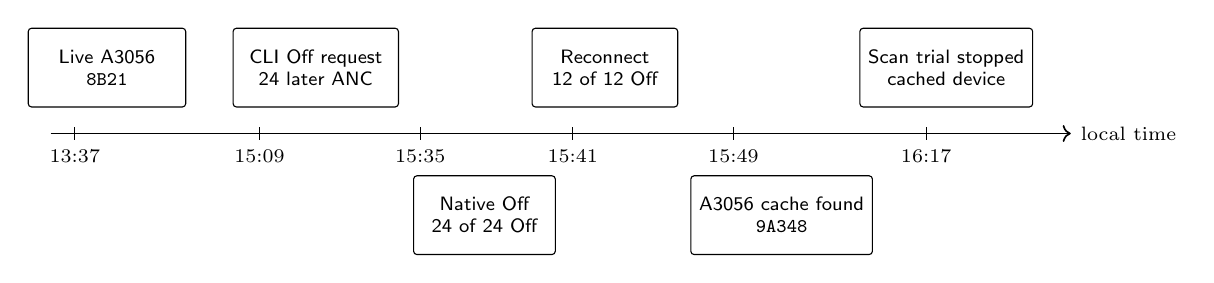
\begin{tikzpicture}[x=1.02cm,y=1cm]
\draw[->,semithick] (0,0) -- (12.7,0) node[right,font=\scriptsize]{local time};
\foreach \x/\l in {0.3/{13:37},2.6/{15:09},4.6/{15:35},6.5/{15:41},8.5/{15:49},10.9/{16:17}}{\draw (\x,0.08)--(\x,-0.08) node[below,font=\scriptsize]{\l};}
\node[phase,minimum width=2cm,above=0.23cm] at (0.7,0.1) {Live A3056\\\texttt{8B21}};
\node[phase,minimum width=2.1cm,above=0.23cm] at (3.3,0.1) {CLI Off request\\24 later ANC};
\node[phase,minimum width=1.8cm,below=0.33cm] at (5.4,-0.2) {Native Off\\24 of 24 Off};
\node[phase,minimum width=1.85cm,above=0.23cm] at (6.9,0.1) {Reconnect\\12 of 12 Off};
\node[phase,minimum width=2.25cm,below=0.33cm] at (9.1,-0.2) {A3056 cache found\\\texttt{9A348}};
\node[phase,minimum width=2cm,above=0.23cm] at (11.15,0.1) {Scan trial stopped\\cached device};
\end{tikzpicture}
\caption{Selected observations through the first controlled preflight on November 7, 2026. Horizontal spacing is schematic and not to scale. Boxes mark host observations, not continuous monitoring.}\label{fig:timeline}
\end{figure}

\subsection{ANC host readbacks differed by intervention}
The first command-line attempt reported Off immediately after applying the setting. Fifteen seconds later, the first passive observation returned Noise Cancellation, and all 24 samples in the two-minute window continued to report that state. In contrast, after a native-interface intervention, 24 of 24 subsequent samples reported Off. The GUI action itself was not time-stamped in the terminal transcript. After a successful reconnect, 12 of 12 samples still reported Off. Two earlier reconnect attempts were incomplete because the script saw only MacBook Pro Speakers. Figure~\ref{fig:anc} reports the valid sample counts by condition, without implying sample independence.

\begin{figure}[htbp]\centering
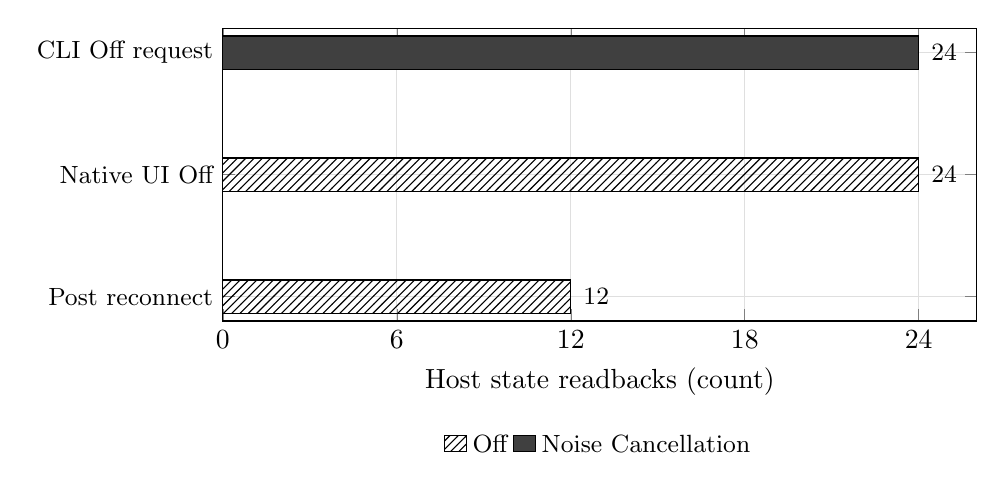
\begin{tikzpicture}
\begin{axis}[
  xbar stacked, width=0.92\linewidth,height=5.3cm,
  symbolic y coords={CLI Off request,Native UI Off,Post reconnect},
  ytick=data, y dir=reverse, xmin=0,xmax=26,
  xlabel={Host state readbacks (count)},
  bar width=12pt,
  legend style={at={(0.5,-0.35)},anchor=north,legend columns=2,draw=none,font=\small},
  yticklabel style={font=\small},
  xtick={0,6,12,18,24}, grid=major, grid style={gray!25},
]
\addplot[xbar,draw=black,fill=white,pattern=north east lines,pattern color=black] coordinates {(0,CLI Off request) (24,Native UI Off) (12,Post reconnect)};
\addplot[xbar,draw=black,fill=black!75] coordinates {(24,CLI Off request) (0,Native UI Off) (0,Post reconnect)};
\legend{Off,Noise Cancellation}
\node[font=\small,black,anchor=west] at (axis cs:24.1,CLI Off request) {24};
\node[font=\small,black,anchor=west] at (axis cs:24.1,Native UI Off) {24};
\node[font=\small,black,anchor=west] at (axis cs:12.1,Post reconnect) {12};
\end{axis}
\end{tikzpicture}
\caption{Sixty host-reported ANC samples under three different observation conditions. Counts indicate repeated reports, not independent trials or independently measured acoustic states.}\label{fig:anc}
\end{figure}

The comparison shows that ANC Off was stable for the observed later windows and across one successful reconnect. Thus, the early discrepancy cannot be interpreted as evidence that ANC invariably re-enables after reconnection. It is consistent with a third-party setting/reporting issue, conditional behavior, or unobserved state changes. Firmware causation was not established.

\subsection{Log volume was dominated by unrelated or ambiguous messages}
One two-hour updater extraction included 3,257 records. A text-based triage excluded 1,515 messages of the form \texttt{Could not remove expired file at <private>; error <private>} from the \texttt{uarpd} host pruner. Another 1,531 messages matched a broad keyword expression, with 211 remaining unmatched. The pruner reports were retained in private evidence, but their filenames and error details were redacted by the operating system. They could not be correlated to the target earbud.

\begin{figure}[htbp]\centering
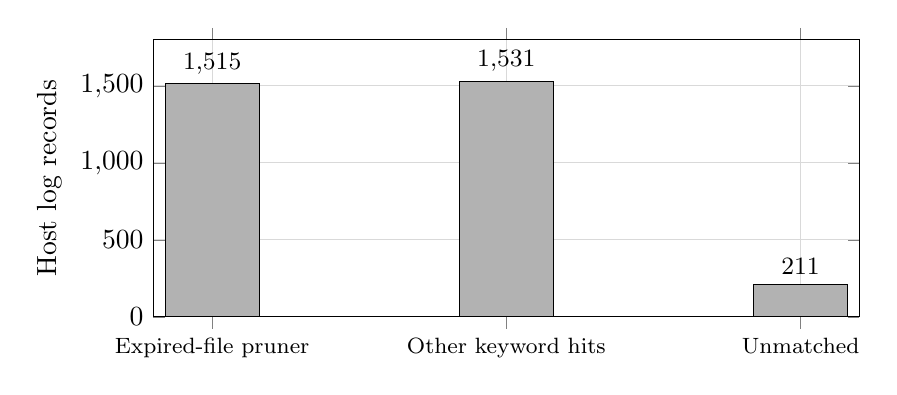
\begin{tikzpicture}
\begin{axis}[ybar,width=0.87\linewidth,height=5.1cm,
bar width=34pt, ymin=0,ymax=1800,
xtick=data, symbolic x coords={Pruner,Other matches,Unmatched},
xticklabels={Expired-file pruner,Other keyword hits,Unmatched},
xticklabel style={font=\footnotesize,align=center},
ylabel={Host log records},
ytick={0,500,1000,1500},grid=major,grid style={black!15},
axis line style={black},nodes near coords,nodes near coords style={font=\small}]
\addplot[fill=black!30,draw=black] coordinates {(Pruner,1515) (Other matches,1531) (Unmatched,211)};
\end{axis}
\end{tikzpicture}
\caption{Host updater log triage. All 3,257 records were partitioned by a documented text filter. These are diagnostic categories, not a measure of defect frequency or device-specific fault attribution.}\label{fig:triage}
\end{figure}

Some records reported that \texttt{com.apple.AUDeveloperSettings.plist} was unavailable. Other subscription lookups reported \texttt{Found asset=(null)} or \texttt{No cached record found}, followed by successful lookups of the same A3056 \texttt{9A348} cache record. The messages may reflect different subscriptions or fallback paths; the available excerpt is insufficient to attribute a specific updater failure. A case-associated log entry contained a generic \texttt{AirPods Pro Case} label, which was treated as a host display label rather than proof of case-hardware mismatch.

\subsection{Historical capture triage (November 6 corpus)}
Two overlapping same-day historical captures (a primary archive and a follow-up extraction) together contained approximately 230 MB uncompressed and 1,467,868 lines. Because the captures overlap in time, they are treated as one corpus, not as independent replications. Within it, explicit \texttt{8B21} mentions numbered 550 in the primary capture and 128 in the follow-up (Figure~\ref{fig:histtimeline}); \texttt{periodicFirmwareCheck} matches numbered 4,291 and 88 under the keyword counting method, while a day-level recount for November 2--6 produced 758, 763, 1,290, 836, and 644 matches (Figure~\ref{fig:fwcheck}); the day-level bars sum to the same 4,291 total and show how the periodic checks distribute across days; 133 primary-capture records reported Bluetooth SQL compilation failures and 10 reported legacy accessory-updater initialization failures; and \texttt{9A348} appeared zero times. The zero-count finding is staged evidence: across the historical window the host updater log shows repeated periodic checks against the then-installed version, with no record of the newer candidate being evaluated for this target. A BLE observation window in the same corpus logged advertising activity across channels 37, 38, and 39 (315, 394, and 409 observations; Figure~\ref{fig:blech}); because the observer did not resolve device identity to the AirPods target, those counts describe the surrounding radio environment, not the target's transmit power.

\begin{figure}[htbp]\centering
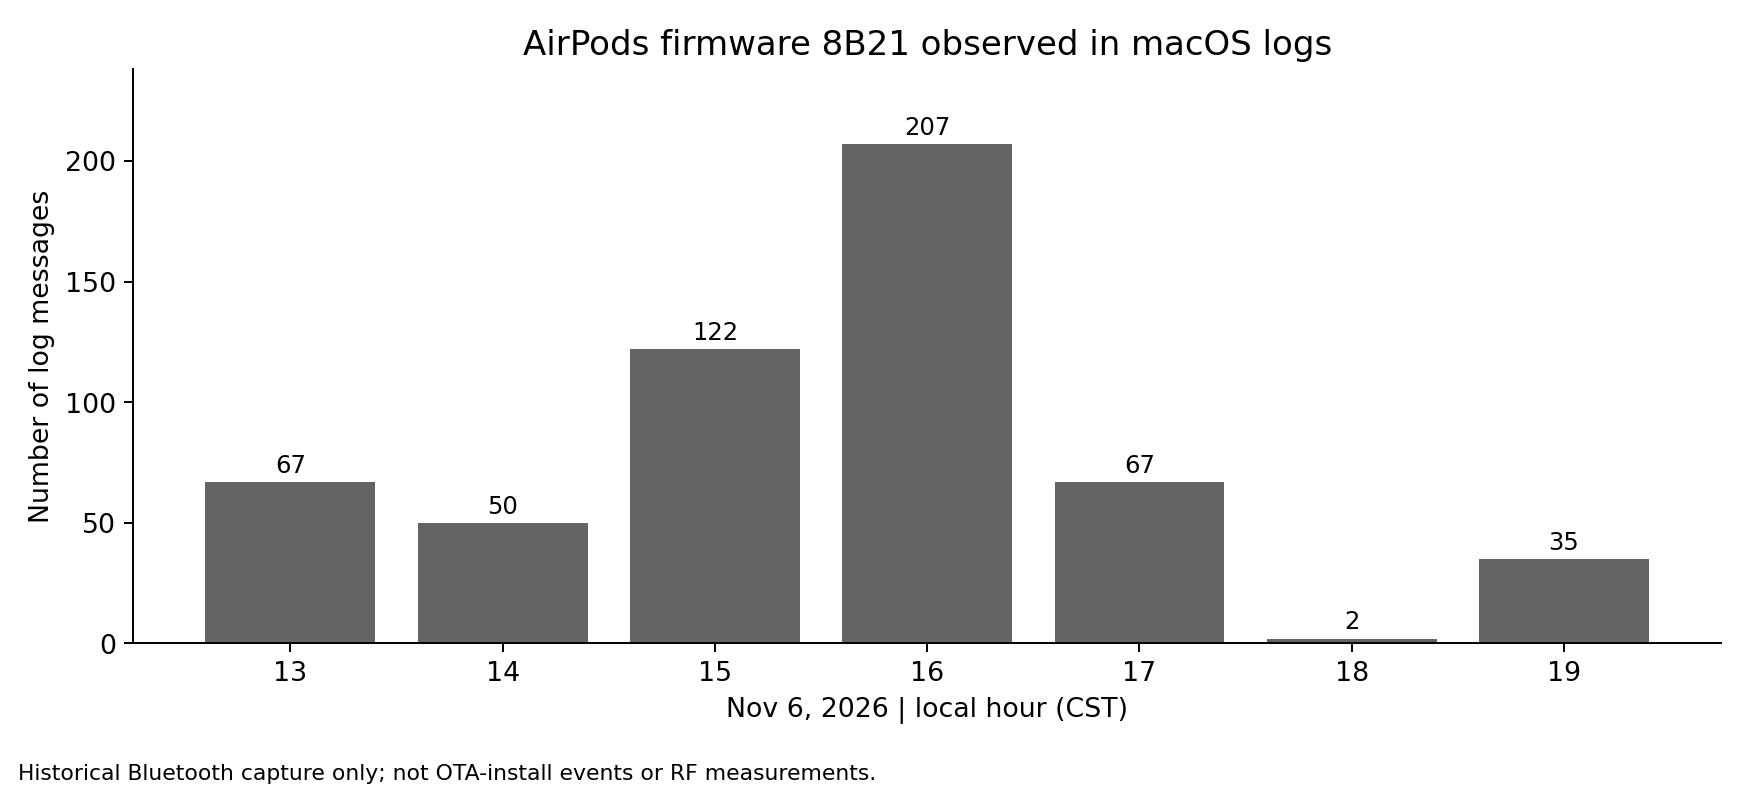
\includegraphics[width=0.94\linewidth]{figures/historical_8b21_timeline_bw.png}
\caption{Hourly count of explicit \texttt{8B21} mentions in the November 6 primary historical capture (67+50+122+207+67+2+35 $=550$). Counts are log-line mentions, not update events.}\label{fig:histtimeline}
\end{figure}

\begin{figure}[htbp]\centering
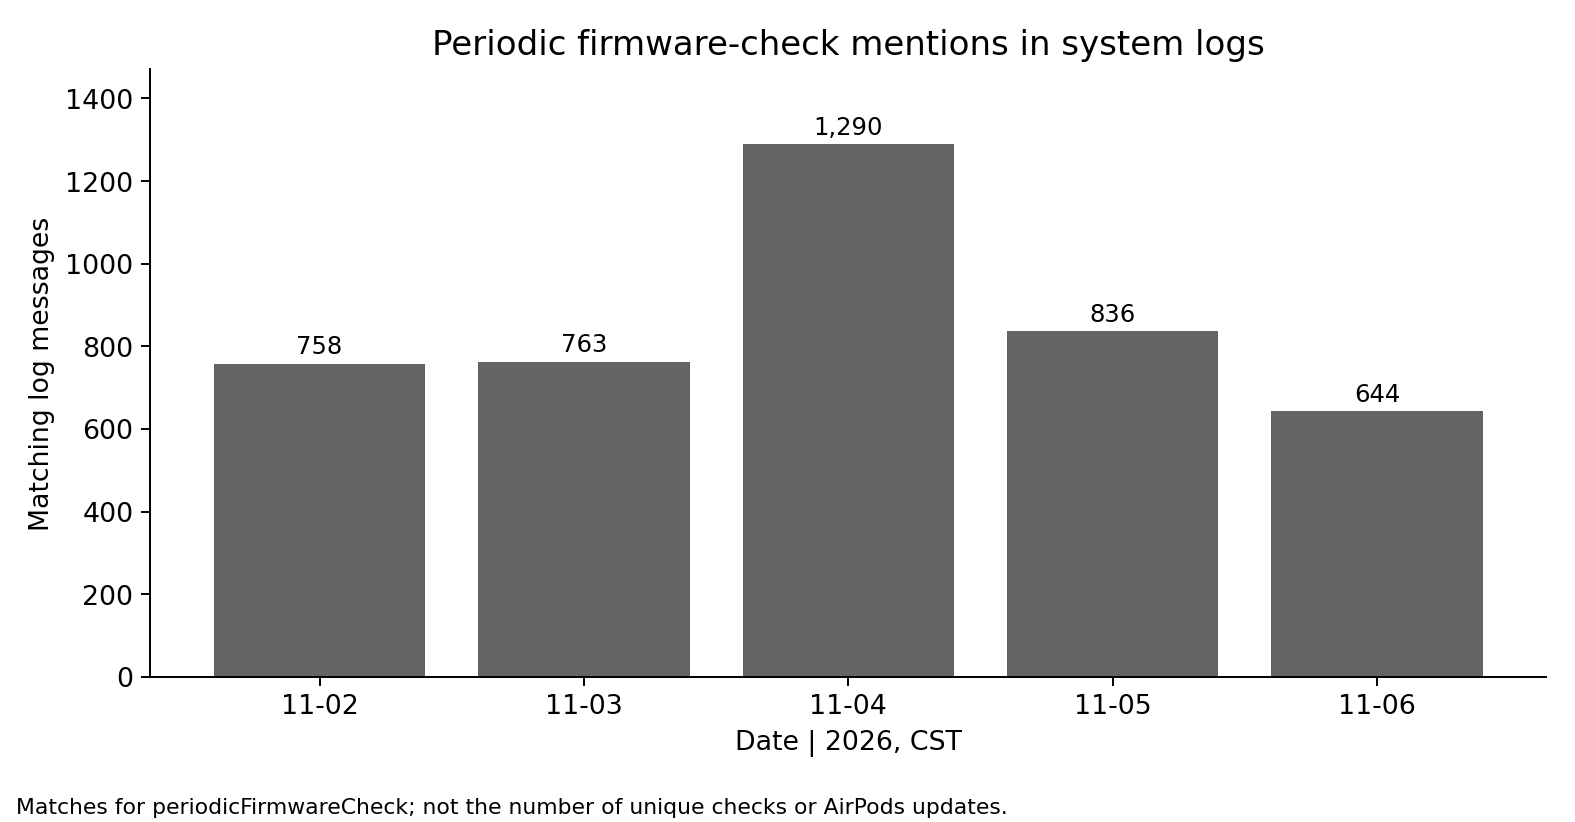
\includegraphics[width=0.94\linewidth]{figures/firmware_check_activity_bw.png}
\caption{Daily \texttt{periodicFirmwareCheck} matches, November 2--6 (758, 763, 1,290, 836, 644). The day-level bars sum to 4,291, matching the keyword-level total in the same corpus; the two distributions differ by day, not by total.}\label{fig:fwcheck}
\end{figure}

\begin{figure}[htbp]\centering
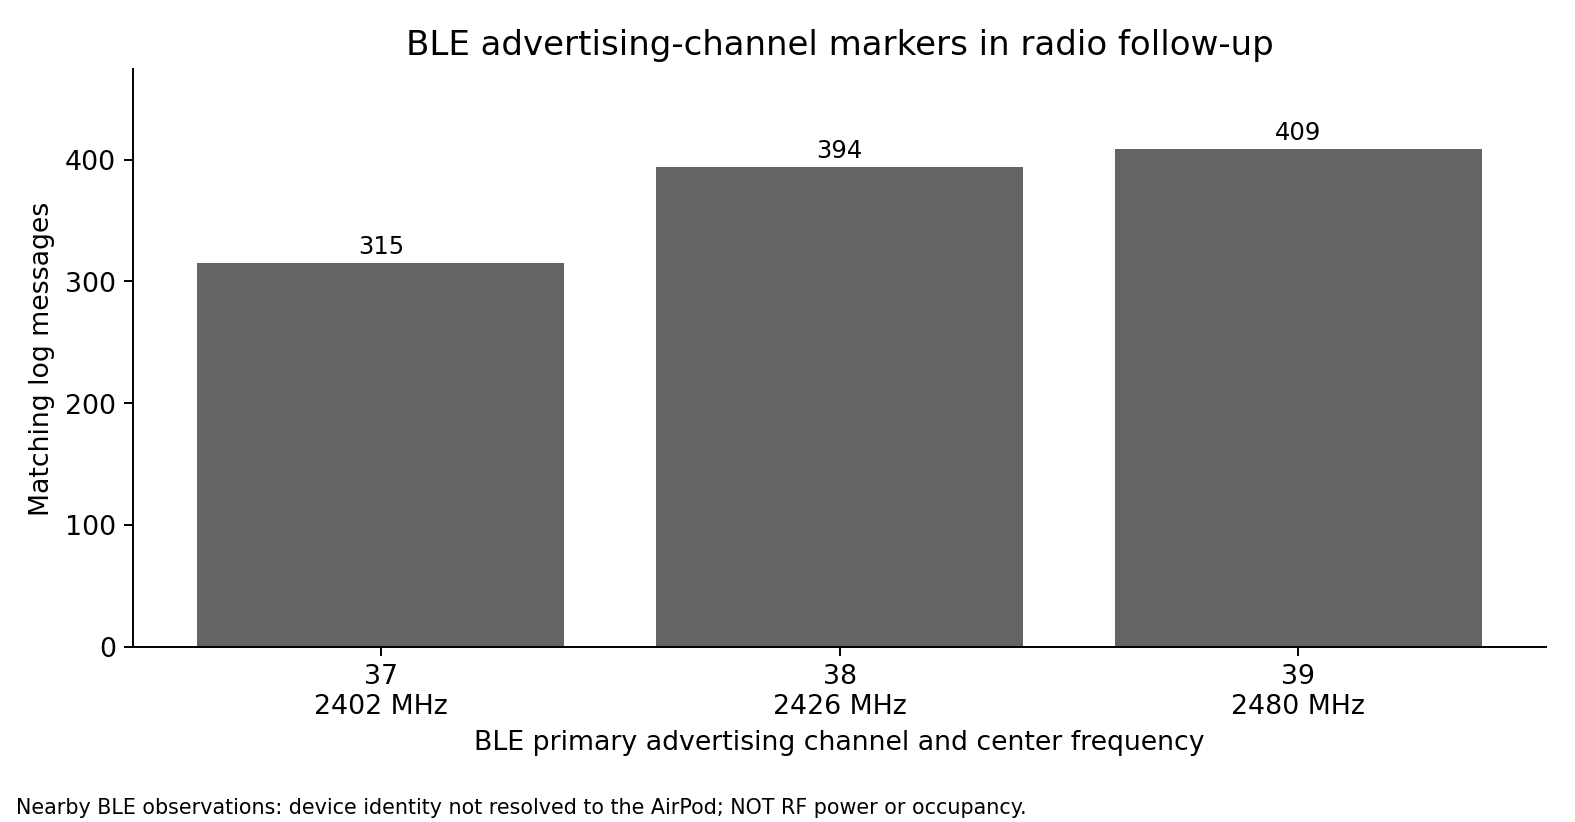
\includegraphics[width=0.94\linewidth]{figures/ble_advertising_channels_bw.png}
\caption{Advertising-channel distribution across a BLE observation window (channel 37: 315, channel 38: 394, channel 39: 409). Device identity was not resolved to the AirPods target; these counts describe the RF environment, not the target's transmit power.}\label{fig:blech}
\end{figure}

\subsection{The first controlled scan trial was blocked by its own preflight}
At 16:17:47, the research trial produced:
\begin{lstlisting}
Product: 0x201B | Live connected: False |
Installed firmware: 8B21
STOP: macOS reports this device DISCONNECTED (cached reading).
Preflight did not pass. No scan request was posted.
\end{lstlisting}
The scan script required an active macOS audio-device connection before posting a scan. When the bud was in the closed case, that prerequisite was not met. Apple's published process requires initial pairing/connection but then explicitly moves the earbuds into a closed, powered case for the maintenance interval \cite{applefw}. The failed preflight therefore exposed a protocol-design problem in the research harness. It did not produce an Apple eligibility verdict and did not test an over-the-air transfer.

\subsection{Experiment F-02: scan posted, connected firmware unchanged}
The corrected manual trial progressed beyond the earlier preflight. Table~\ref{tab:f02} preserves the distinction between an update request, cached queries, and a subsequent connected-device reading.
\begin{table}[htbp]\centering\small
\caption{Experiment F-02: bounded post-scan observations on November 7, 2026 (CST). The scan timestamp was not printed in the supplied output.}\label{tab:f02}
\begin{tabularx}{\linewidth}{@{}p{0.19\linewidth}p{0.27\linewidth}X@{}}\toprule
Time & Host interface & Observation \\ \midrule
16:17:47 & Original preflight script & Disconnected/cached \texttt{8B21}; script stopped; no scan posted in this first trial. \\
Not recorded & Manual \texttt{airpods-fw update} & One system-wide Apple scan notification successfully posted. \\
16:47:33 & \texttt{airpods-fw status/check} & Disconnected/cached; earbud and case \texttt{8B21}; 100\% battery. \\
16:48:27 & \texttt{airpods-fw status} & Disconnected/cached; earbud and case \texttt{8B21}. \\
16:49:43 & \texttt{airpods-fw status} & Connected target \texttt{0x201B}; earbud and case \texttt{8B21}; 100\% battery. \\
Immediately after & \texttt{system\_profiler} & Connected target \texttt{0x201B}; earbud and case \texttt{8B21}. \\
\bottomrule\end{tabularx}
\end{table}

The observed intervention outcome was \emph{no firmware-version progression during the bounded trial}. The version was obtained from a connected session following a successfully posted scan request. The available host log excerpts did not establish an A3056-correlated transfer attempt, completed activation, or explicit rejection decision. The missing companion earbud is one explanatory hypothesis requiring an eligibility trace or a controlled comparator.

\subsection{Bounded direct-transport diagnostics: what the accessory answered}\label{sec:transport}
Table~\ref{tab:transport} summarizes every preserved direct-transport run. Four findings survive scrutiny.

\begin{center}\small
\begin{longtable}{@{}p{0.10\linewidth}p{0.19\linewidth}p{0.23\linewidth}p{0.38\linewidth}@{}}
\caption{Preserved direct-transport runs, November 7, 2026 (CST). Every run was information-only except the three operator-authorized offer sessions (F-08T/U/V), which each transmitted one offer referencing the cached candidate image; acknowledgments and terminal processing events were client-decoded, and F-08U/V flags require qualified interpretation; no run transmitted a transfer, staging, or apply command.}\label{tab:transport}\\
\toprule Time & Experiment & Target state & Outcome \\ \midrule
\endfirsthead
\multicolumn{4}{@{}l}{\footnotesize Table \ref{tab:transport} (continued)}\\[2pt]
\toprule Time & Experiment & Target state & Outcome \\ \midrule
\endhead
\midrule \multicolumn{4}{r@{}}{\footnotesize(continued on next page)}\\
\endfoot
\bottomrule
\endlastfoot
17:21--17:39 & F-05, F-05B, F-05C & Advertising / GATT connected & One Apple-manufacturer candidate labeled as AirPods (RSSI $-43$ dBm in the public CSV); UARP characteristic found under service \texttt{4715650B-5E9D-}\allowbreak\texttt{4AC2-B898-}\allowbreak\texttt{A4FC0AA5DF78}; PnP ID \texttt{0x004C}/\texttt{0x201B} exact match; model A3056; firmware characteristic present but not decoded. \\
17:35 & F-05D run 1 & GATT connected & Six UARP information frames transmitted (sync, protocol version, running tag 5, staged tag 6, update statistics tag 7, last error tag 8); zero replies; session closed by gate. \\
17:38 & F-05D run 2 & Two candidates & Uniqueness gate failed; stopped before any write. \\
17:39 & F-05E & GATT connected & UARP sync and protocol-version writes acknowledged (2 ACK, 0 rejected); no UARP indication received; session closed by gate. \\
(not preserved) & F-04, F-06 & Host-side & F-04: read-only cached-payload parse, 17/17 payloads bounds-valid, \textsc{ftab} SHA-256 match. F-06: Calvados reference probe not runnable on this host (no \texttt{dbus}/\texttt{bluetoothctl}; Docker VM exposes zero Bluetooth adapters). \\
18:15 & F-08T & Paired, disconnected at lid open & L2CAP PSM \texttt{0x1001} open (MTU 672) at 5.0 s; AAP handshake TX; UARP sync RX; protocol v4 negotiated; accessory answered queries: running firmware \texttt{8.1.21.0}, staged \texttt{0.0.0.0}; \texttt{9A348} offer TX; \textbf{offer acknowledged; client-decoded abandoned} (reason 0); channel closed at 7.7 s; no image data requested. \\
18:29 & F-08U & Paired, disconnected; AACP settle gate ($\geq$6 s) & Same session structure; running \texttt{8.1.21.0}, staged \texttt{0.0.0.0} confirmed by accessory; offer TX; \textbf{acknowledged; terminal flags \texttt{0x0003}} (denied/abandoned ambiguous); no image data requested. \\
18:30 & F-08V & Same as F-08U & Same raw terminal flags; third acknowledged offer without image-data request. \\
18:49--19:04 & F-08T later windows (3), F-09 windows (5) & Connected / conditioned lid window & Every L2CAP open failed \texttt{0xE00002BC} (18:56:45, 19:02:30, 19:04:26 for the later F-08T windows); two F-09 windows stopped at the connected-target check; nothing sent. \\
18:59 & F-08X gate & Disconnected & Battery-telemetry gate found zero connected \texttt{0x201B} records; stopped before transport. \\
18:59--19:00 & F-10 check/offer & Paired, disconnected & Native baseband reconnect attempt returned \texttt{0xE00002D6} after 20.1 s; no UARP offer. \\
19:07 & F-11 & Connected & Single L2CAP open attempt failed \texttt{0xE00002BC} at 3.2 s; no retry, no disconnect issued. \\
19:10 & F-12 & Connected & Precondition check: target already connected; no traffic. \\
19:12 & F-12B run 1 & Paired, disconnected & One L2CAP PSM \texttt{0x1001} open succeeded (outgoing MTU 672); AAP control handshake send failed \texttt{0xE00002E7}; channel closed. \\
19:13 & F-12B run 2 & Paired, disconnected & Channel open (MTU 672); AAP handshake transmitted and acknowledged; AACP notification registration, UARP sync, and UARP version request transmitted; no valid UARP version reply; accessory closed the channel at 21.5 s. \\
19:17--19:49 & F-13 (6 attempts) & Lid closed & Target remained CONNECTED through each 120 s wait; never entered DISCONNECTED; no L2CAP or UARP traffic. \\
\end{longtable}
\end{center}

First, \textbf{device identity is unambiguous over GATT.} The PnP ID read returned vendor \texttt{0x004C} and product \texttt{0x201B}, the model string contained A3056, and the serial-number characteristic was never queried. The UARP GATT characteristic was present with write and indication properties. A two-candidate scan failed the uniqueness gate and was stopped, which is the intended behavior when a second Apple audio accessory is advertising.

Second, \textbf{the accessory accepted writes but returned no UARP indication within the bounded observation window.} In F-05E, both information writes were acknowledged at the ATT layer and none were rejected, yet zero UARP indications arrived during the bounded response window; the experiment does not establish that a response is impossible under other conditions. An acknowledged GATT write establishes transport delivery to the accessory's BLE stack, not that the accessory's UARP state machine consumed the message.

Third, \textbf{control-channel reachability depends on host connection state.} From a connected Apple-host audio state, the L2CAP AAP control channel was unavailable across every variant (single open, retry loops, conditioned lid-window protocols), with a consistent IOKit failure result. From a paired-but-disconnected state, channel opens did succeed: in the minimal F-12B design, the case lid opening triggered the open, the AAP handshake was acknowledged on the second attempt, and UARP sync and version-request frames were transmitted, but no valid UARP version reply arrived before the accessory closed the channel 21.5 seconds after the open; the fuller F-08T/U/V sessions on the same channel were answered end to end (detailed in the next subsection). A final diagnostic showed the target holding a CONNECTED state for more than two minutes with the case lid closed, so the paired-disconnected precondition itself was the scarce resource.

Throughout the series, cached right-earbud battery telemetry drifted between unavailable, a phantom 57\% at approximately 18:40 (reported for a bud that is physically lost), and 1\% across runs. That instability is consistent with a missing companion and confirms that host battery telemetry is not proof of physical earbud presence; it was treated accordingly, motivated the right-bud-gated F-08X design, and was never used as an eligibility signal.

\subsection{Experiments F-08T/U/V: answered UARP sessions and terminal offer-processing events}
Fourth, \textbf{the accessory answered the session and issued terminal offer-processing notifications after acknowledging the offers.} Three authorized sessions reached a stage no earlier run reached: a live, answered UARP session with the accessory's own endpoint. In F-08T (18:15:09), the control channel opened 5.0 seconds after lid-open from a paired-but-disconnected state (outgoing MTU 672, after two short disconnects). The AAP handshake was transmitted, a UARP sync was received from the accessory, protocol version 4 was reported as negotiated (the host-proposed version is not recoverable from the public supplement), and the accessory \emph{answered} the information queries: it reported running firmware \texttt{8.1.21.0} and staged firmware \texttt{0.0.0.0}, the first device-confirmed version readbacks of the study; the numeric UARP version \texttt{8.1.21.0} is consistent with the short \texttt{8B21} build designation under a naming convention documented for sibling hardware \cite{calvados}; this format correspondence is not firmware-installation attestation. The staged-version field \texttt{0.0.0.0} records what the accessory reported at query time and does not by itself exclude an earlier or out-of-band staging operation. The offer I authorized referencing the cached \texttt{9A348} build was then transmitted; the accessory \textbf{acknowledged the offer} and the client subsequently decoded an \emph{offer abandoned} message (reason 0), closing the channel 7.7 seconds after open. No transfer request followed: the accessory never asked for image data. The protocol events of these three sessions were reconstructed from the experimental client's own logs and decoder; an independent full HCI or PacketLogger capture of these exact sessions was not obtained, so the recorded messages are client-decoded observations rather than independently corroborated on-air captures.

F-08U (18:29:03) and F-08V (18:30:33) repeated the session with an added AACP settle gate that held the open channel for at least six seconds before any UARP traffic, to test whether the earlier client-classified terminal response was sensitive to session timing. Both sessions again produced running \texttt{8.1.21.0}, staged \texttt{0.0.0.0}, an acknowledged offer, and a terminal processing notification with flags \texttt{0x0003}, which the local client labeled abandoned. The value is not uniquely classifiable from the released evidence: the Calvados UARP notes also describe a denied status combined with reason 1 as \texttt{0x0003} \cite{calvados}. The settle gate did not change the recorded raw value. In all three sessions the client recorded a terminal offer-processing event before the transfer stage; no image bytes moved in either direction.

The preserved record also shows the harness converging on this result: an early F-08 variant stopped on an unexpected UARP payload-table structure, F-08R stopped when zero paired devices matched the verified A3056 name, F-08S stopped on an unexpectedly resolved device address, and every later conditioned attempt (later F-08T windows at 18:56:45, 19:02:30, and 19:04:26, and the F-09 windows) failed to open the channel at all (\texttt{0xE00002BC}), so nothing was sent. My hypothesis, recorded in the F-09 protocol header, was that the 18:15 terminal response occurred because the offer arrived outside the window in which the bud accepts offers; that hypothesis is reported here as a hypothesis, not a finding.

\section{Update Initiation and the Workaround Boundary}\label{sec:intervention}
\subsection{Available host tools}
The open-source \texttt{airpods-fw} utility can inspect known device firmware, retrieve Apple release and catalog metadata, inspect local asset records, request an accessory scan, and observe macOS updater logs \cite{airpodsfw}. Its \texttt{update} implementation verifies a launchd notification registration and executes \texttt{notifyutil -p com.apple.SoftwareUpdate.ScanTriggered}. The source does not implement an image-transfer operation or device-specific flashing session. The \texttt{--device} flag limits the tool's displayed or monitored target; the Apple notification is system-wide. Its \texttt{--watch} mode also requires a fresh connected-device version report to declare success, which can be unavailable for most of the closed-case interval.

The installed \texttt{pods-control} utility pertains to audio accessory settings and is not a firmware updater. A payload-inspection utility can parse image metadata but cannot by that fact deliver an authenticated image to hardware. The research distinguishes observation utilities, scan triggers, and actual firmware-transfer mechanisms because confusing these capabilities would create a false positive in the experimental outcome.

The bounded direct-transport series adds the corresponding boundary on the other side: even where a raw channel exists, the information-only sessions stopped before any offer-bearing stage, and the three authorized offer sessions (F-08T/U/V) stopped before any image-data request, transfer, staging, or apply message; in each session the client recorded an offer acknowledgment followed by a terminal processing notification, with the F-08U/V status still ambiguous. The presence of an Apple-signed cached image on the host plus an open control channel is therefore still not an update path; transport, protocol acceptance, and policy all remain separate stages.

\subsection{Corrected case-closed scan experiment}
The corrected protocol separates an initial evidence snapshot, a system-wide scan notification, a case-closed observation interval, and subsequent live verification. In the reported trial, I ran the dry-run and scan commands directly; the public script codifies the same sequence for replication and records timestamps when used. It posts no more than one notification per invocation. It does not select a firmware file, write a system cache, or bypass a device trust mechanism.

\begin{figure}[htbp]\centering
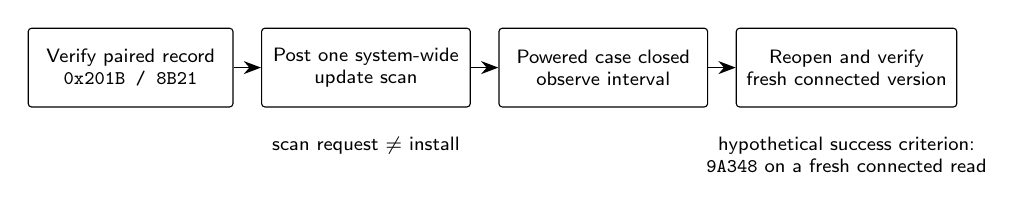
\begin{tikzpicture}[node distance=0.35cm]
\node[phase,minimum width=2.6cm] (p) {Verify paired record\\\texttt{0x201B / 8B21}};
\node[phase,minimum width=2.65cm,right=of p] (n) {Post one system-wide\\update scan};
\node[phase,minimum width=2.65cm,right=of n] (w) {Powered case closed\\observe interval};
\node[phase,minimum width=2.8cm,right=of w] (v) {Reopen and verify\\fresh connected version};
\draw[arr] (p)--(n);\draw[arr] (n)--(w);\draw[arr] (w)--(v);
\node[font=\sffamily\scriptsize,below=0.25cm of n] {scan request $\ne$ install};
\node[font=\sffamily\scriptsize,align=center,below=0.25cm of v] {hypothetical success criterion:\\ \texttt{9A348} on a fresh connected read};
\end{tikzpicture}
\caption{Corrected update experiment. A cached paired-device record is sufficient to select a local research target; it is not treated as proof that the peripheral is currently reachable. The only requested action is the Apple scan notification.}\label{fig:protocol}
\end{figure}

\begin{enumerate}[leftmargin=2em]
\item Record the paired target \texttt{0x201B}, its cached firmware version, and the date. Ensure the Mac has Bluetooth and Wi-Fi enabled. If a live reading is accessible before closing the lid, preserve that observation.
\item Place the surviving left earbud in its original charging case, connect the case to USB power, close the lid, and keep the case within Bluetooth range of the Mac.
\item Post one Apple system-wide accessory scan using \texttt{python3 airpods-fw update --device 0x201B}. Capture the exit code and exact local timestamp.
\item Leave the case closed for at least 30 minutes, consistent with Apple's public charging-case update sequence \cite{applefw}. Do not require a continuous active audio connection during this interval.
\item Open the case, reconnect the target, and obtain fresh firmware state from \texttt{system\_profiler} and \texttt{airpods-fw status --device 0x201B}. Preserve whether the readback is connected or cached.
\item Extract a bounded macOS updater log window around the scan timestamp. Remove serial numbers, MAC addresses, pairing tokens, and unrelated devices before public release.
\end{enumerate}

\paragraph{Outcome rule.} A fresh connected report of \texttt{9A348} for product \texttt{0x201B} constitutes host-confirmed version progress. A posted notification followed by a fresh connected \texttt{8B21} readback is classified as \emph{no version progression observed in the trial}. A cached-only readback remains indeterminate. A trace containing a targeted eligibility denial or transfer error should be recorded verbatim and evaluated on its own terms. A generalized single-earbud prohibition requires evidence beyond one case.

\paragraph{Current disposition.} The manual corrected scan request was posted successfully. At 16:49:43, the connected A3056 and case remained on \texttt{8B21}; \texttt{system\_profiler} corroborated this version and connection state. The intervention result is therefore recorded as no observed version progression, with the updater eligibility and transfer mechanism unresolved.

\section{Interpretation and Validity Threats}\label{sec:validity}
\subsection{Why a local asset is not a firmware installation}
The difference between \texttt{9A348} in the host cache and \texttt{8B21} in accessory records is a useful finding precisely because it isolates a stage boundary. The host can store an image without having selected a particular target, negotiated transport, passed eligibility, written an image, or verified activation. The observed \texttt{UARPAssetCacheRecord} and \texttt{UARPEndpointPersonalityMobileAsset} messages do not contain a transfer acknowledgement. The inference \emph{firmware exists, therefore the earbud must be able to install it} is not warranted.

\subsection{Missing right member as a hypothesis}
The lost right earbud is the most salient difference between this configuration and a standard complete pair. That makes a companion-dependency hypothesis worth testing. However, the current data include no Apple-recorded rejection reason tying update refusal to the absent member, no successful paired A3056 control under comparable conditions, and no proof that all normal host conditions were satisfied during previous extended charging. The post-scan connected readback strengthens the observation of a persistent version gap. The missing-earbud mechanism remains a research hypothesis with a clear next experiment, not a verified policy.

The adjacent-hardware evidence sharpens rather than resolves H1. On AirPods Pro 2 (USB-C), the case-mediated completion path demonstrably requires both buds, while the host-driven staging path demonstrably does not \cite{calvados}. If macOS's updater relied on case coordination for a one-bud A3056 set, a missing companion could plausibly stall completion; if it uses the host path, the missing companion is not architecturally a necessary blocker. Calvados also documents applying a staged image on its primary bud without a synchronized secondary-bud update; this sibling-hardware behavior does not establish an A3056 capability or an operation performed here \cite{calvados}. Which path macOS attempts for this configuration is exactly the eligibility question this study marks unresolved, and no A3056-specific evidence exists either way.

\subsection{Transport gating as a bounded observation}
Calvados documents differences between AAP-tunneled session holds and GATT behavior on AirPods Pro 2, but also demonstrates that GATT UARP can successfully carry firmware data on that sibling model \cite{calvados}. Accordingly, the present A3056 observations cannot establish that the AAP-tunneled channel is inherently privileged for information queries. This study examined the Apple-host path under bounded conditions. The control channel was unreachable from a connected audio state across every variant; the minimal F-12B session that did open produced no UARP answer; and the later, fuller F-08T/U/V sessions on the same channel were answered end to end, including device-confirmed version readbacks, which indicates that the F-12B silence reflects the minimal session the F-12B probe offered rather than fundamental reachability. The F-05E GATT silence (two ATT acknowledgments, zero UARP indications) cannot distinguish missing response framing, an incomplete session, and other transport or firmware-state conditions. Calvados documents a required one-byte fragment prefix on its sibling-hardware GATT UARP channel. The original A3056 GATT probe source was not deposited, so the presence and correctness of that prefix cannot be verified from the public CSV. Three readings of the F-12B result remain possible: the accessory's UARP endpoint requires a session-establishment step that probe did not implement; the endpoint answers only sessions initiated by Apple's own updater; or the endpoint answered and the reply was lost at a layer the probe did not instrument. The F-08T/U/V sessions, which implemented the fuller handshake, were answered; the evidence does not select among the remaining explanations for the F-12B window specifically. What the series establishes is narrower and still useful: a single-bud A3056 exposes an identity-verifiable GATT surface, acknowledges information writes on it, exhibits state-dependent control-channel reachability, and conducts an answered UARP v4 session on the AAP-tunneled channel, without proceeding to image-data requests, transfer, staging, or Apply in the recorded offer sessions.

\subsection{Offer acknowledgments, ambiguous terminal flags, and unresolved state}
The F-08T/U/V sessions move the evidence boundary: the client recorded accessory-originated UARP running-version and staged-version responses, one acknowledged firmware offer per session, and a subsequent terminal processing notification before any image-data request. In F-08T the client reported abandonment with reason 0. In F-08U and F-08V the recorded flags were \texttt{0x0003}; the local decoder labeled them abandoned, while Calvados also identifies \texttt{0x0003} as a possible denied status with reason 1 on sibling hardware \cite{calvados}. The value \texttt{0x0003} alone cannot distinguish these two bitwise encodings. Original decoder code, state context, and independent packet evidence are needed for stronger classification, and even those may not resolve the collision without additional context. Both F-08U/V offers followed a settle gate of at least six seconds. The accessory never requested image data, so the transfer stage was never reached; apply was never sent; the installed image was untouched. These are the only recorded terminal offer-processing notifications in the bounded series. Earlier accessory-originated events, including GATT write acknowledgments, UARP information responses, and offer acknowledgments, had already been observed. The raw terminal values alone do not establish why processing stopped: it does not by itself establish an eligibility policy, a companion-bud dependency, a signature rejection, or an offer-window condition. The recorded reason fields do not discriminate among offer-window timing, companion-bud policy, case or battery gating, a model-specific filter, an implementation or decoding defect, and stale UARP session state. On AirPods Pro 2, Calvados observed that closing and reopening a charging case reset offer state and changed a refused offer into an accepted one \cite{calvados}. The present three offers occurred close together without a documented equivalent state-reset control, so that alternative remains open; the two settle gates do not test it. The cause and any associated eligibility decision remain unresolved. What the sessions do exclude is narrower: a control-channel transport failure is not the blocker for session establishment and control-message exchange when the channel is open and answered, and the specific asset-integrity failures tested in F-04 are not supported by its structural findings. The image-transfer path itself was not exercised, so no downstream transfer failure mode is excluded. Resolution would require original raw-frame and decoder reconciliation, a separately authorized state-reset comparison under controlled charging and case conditions, or a vendor eligibility statement. No such additional experiment was performed here.

\subsection{Sampling, cached data, and tool measurement}
The 60 ANC samples were repeated host observations within a small number of test sessions, not 60 independent devices or 60 randomized trials. Their aggregate supports the narrow statement that the host repeatedly reported different settings after different intervention methods. It cannot estimate a population failure rate. The reconnect prompts record operator actions; the return key alone cannot prove Bluetooth attachment, which is why two attempts were excluded. Similarly, a disconnected host record may be stale. The final connected \texttt{airpods-fw} and \texttt{system\_profiler} readings reduce this uncertainty for the bounded trial, but may still share host firmware metadata. A first-party GUI control is not a calibrated external microphone measurement of ANC output.

\subsection{Reported ear discomfort and physical exposure}
I reported ear discomfort and headaches during use and chose to avoid further wear. Firmware affects software-controlled audio behavior, so a relationship can be considered as a testable question. The current study did not measure acoustic output, eardrum sound-pressure exposure, fit, temperature, radiofrequency transmission power, specific absorption rate, or physiological response. Bluetooth RSSI is received signal strength at the Mac, not a measurement of power absorbed by tissue. The symptom report is recorded as motivation and a user observation; its cause is outside the present experimental result.

\subsection{Other limitations}
The test uses one surviving left unit, one associated case, and one Mac. I do not have a complete-pair A3056 comparator, device firmware debug output, a known-good service update, a repeated trial across different hosts, or full unredacted internal eligibility messages. Logs were collected after some events and system privacy redaction obscured the underlying filename and error of numerous pruner messages. Publication timestamps and file modification dates describe host-side artifacts, not peripheral installation times. The manual F-02 scan timestamp was not preserved, so that trial's dwell time is unauditable; the direct-transport series partially compensates by bounding what the transport layer would have shown, but it cannot retroactively complete the scan experiment. Available client-decoded messages do not constitute an independent full HCI packet capture. These constraints determine the scope of the conclusions.

\section{Research Implications and Follow-up Work}\label{sec:implications}
The main technical gap is observability. Users can see an installed version and Apple publishes a newer version, but normal interfaces do not provide a detailed state history such as \emph{asset downloaded}, \emph{candidate selected}, \emph{target ineligible}, \emph{transfer deferred}, or \emph{activation complete}. This matters whenever a user has a partially functional product, including a single surviving earbud, because an unresolved version difference is difficult to diagnose without service-level tools.

A maintainability improvement would be a documented policy for updating one remaining AirPod, together with an explicit per-device reason if the update cannot proceed. A service diagnostic could report which component is missing, the candidate firmware release, and whether pairing, case state, battery, or transport eligibility prevents the operation. A user-visible last-attempt timestamp would distinguish a failure to initiate from a later transfer failure. Apple's documented service-update appointment path is the correct channel for a surviving single bud today, and whether that path accepts one is an open, vendor-answerable question \cite{applefw,applehelp}.

Future tests should compare a complete AirPods 4 ANC pair with a deliberately isolated single member under otherwise identical conditions, using only owner-controlled hardware. A replicating investigator should record initial and final connected versions, case power, lid state, host OS version, Bluetooth proximity, time spent closed, and target-correlated UARP events. Repeated conditions should vary one prerequisite at a time. An iPhone-hosted run of Apple's documented procedure would remove the macOS host as a confound. If Apple can supply a device-specific eligibility result or a supported single-earbud service update, that observation would resolve the leading hypothesis far more efficiently than repeated scan notifications.

\section{Conclusion}\label{sec:conclusion}
The surviving AirPods 4 ANC A3056 continued to report firmware \texttt{8B21} while Apple's current model-family release was \texttt{9A348}. macOS retained the newer A3056 firmware asset and registered the earbud and case as updater endpoints. A first scan trial was invalidated by an overly restrictive host-side connection preflight. The corrected manual sequence posted a system-wide scan request; the preserved transcript did not record the scan timestamp, so the case-closed dwell time cannot be reconstructed, and the trial is classified as no observed version progression with unauditable dwell. Two cached reads and a 16:49:43 connected read still showed \texttt{8B21}; a second host interface corroborated the connected result. Earlier ANC tests demonstrated host-state differences between intervention methods but did not isolate firmware as their cause.

The bounded direct-transport series then established, without ever transferring firmware, that the accessory is identity-verifiable over GATT, acknowledges UARP information writes on the GATT path, opens its L2CAP AAP control channel only from a paired-but-disconnected state, and, in three bounded authorized sessions, reported running firmware \texttt{8.1.21.0} with a staged-version readback of \texttt{0.0.0.0} at query time, acknowledged an offer referencing the cached \texttt{9A348} build, and produced client-decoded terminal processing notifications before requesting any image data. The raw \texttt{0x0003} flags in F-08U/V admit both abandoned and denied interpretations under published sibling-hardware decoding notes. The reviewed evidence contains no confirmed A3056-correlated transfer, activation, or eligibility verdict; the terminal classification and cause remain unresolved.

The experiment establishes a persistent firmware-version gap following a successfully posted host scan and a connected verification, plus state-dependent accessory transport behavior and accessory-originated offer acknowledgments followed by client-decoded terminal responses. Within the direct-offer path, the observed boundary is sharp: the accessory acknowledged each offer and emitted a terminal processing response at or after offer evaluation and before any recorded transfer request; the two \texttt{0x0003} notifications remain ambiguously decoded. Whether Apple's normal updater for this configuration reaches the same stage, or stops earlier for a different reason, is not established by this evidence. Resolving it requires a target-specific Apple eligibility or transfer diagnostic, a vendor service-path statement for a single surviving bud, a matched comparison isolating the second earbud, or an instrumented repetition of the bounded offer session that discriminates among the candidate explanations for these terminal outcomes, including stale session state and protocol decoding.

\section*{Data Availability and Reproducibility}
The publication supplement contains the LaTeX manuscript source, de-identified ANC observations, selected sanitized UARP events, a consolidated direct-transport run table, a one-scan update protocol, and an explicit provenance inventory. The package is mirrored in a GitHub repository that will be made public upon Zenodo deposit, and this preprint is intended for deposit on Zenodo, where versioned updates should be issued as new versions rather than replaced files \cite{zenodoversion}. Original macOS diagnostics contain device identifiers and remain private. The public package supports recomputable counts and data summaries, reusable diagnostic procedures, and sanitized experimental outcomes. Protocol-level reproduction of the direct-transport offer sessions additionally requires the native probe and decoder implementation and the private original transcripts, which are not part of this package. The F-02 connected outcome is preserved in a separate public CSV containing six evidence records with time-precision labels. The transport-trial CSV contains 22 consolidated records representing protocol sessions, grouped attempts, and host-state observations, not 22 independent experiments. Future results should be appended as dated experiments rather than replacing this observation.

\section*{Independence and Research Ethics}
The work was conducted independently using the author's own accessory and Mac, with no third-party device manipulation. The study requested host accessory scans using an existing operating-system interface and did not attempt authenticated firmware bypass, arbitrary device writes, or modifications to Apple-distributed assets. Across every direct-transport run, no image transfer, staging, or apply/reboot command was transmitted; information-only runs transmitted no offer; the three authorized offer sessions each transmitted one offer referencing the cached candidate image, followed by offer acknowledgment and client-decoded terminal processing events (with ambiguous \texttt{0x0003} classification in F-08U/V), with no image data requested or sent; and the cached Apple-signed firmware image was never modified or redistributed. The earbud was not required to be worn during firmware experiments. The reported symptoms are not a clinical finding. The title-page cutaway is an AI-generated conceptual illustration, not a device measurement, radiograph, or representation of verified A3056 internal anatomy.

\section*{Acknowledgment}
The author acknowledges the availability of Apple's public firmware reference, the open-source \texttt{airpods-fw} project, and the Calvados and LibrePods projects' published analysis as independent reference material. Independent technical review is also acknowledged. All responsibility for the experiment design, interpretation, and publication rests with the author.

\begin{thebibliography}{9}
\bibitem{applefw} Apple Inc. ``About firmware updates for AirPods.'' Apple Support, document 106340. Accessed November 7, 2026. \url{https://support.apple.com/en-us/106340}.
\bibitem{airpodsfw} mooons. ``airpods-fw: macOS CLI to inspect AirPods firmware and request Apple's accessory-update scan.'' Source repository, accessed November 7, 2026. \url{https://github.com/mooons/airpods-fw}.
\bibitem{calvados} kronerm. ``Calvados: AirPods firmware research and tooling, including static analysis of build 9A348 (documentation in \texttt{docs/firmware.md}) and a reported AirPods Pro 2 (USB-C) update from 7.1.21 to 9.0.348.'' Source repository, pinned to commit \texttt{caa1113}, accessed November 2026. \url{https://github.com/kronerm/calvados/blob/caa1113/docs/uarp.md} and \url{https://github.com/kronerm/calvados/blob/caa1113/docs/firmware.md}.
\bibitem{librepods612} LibrePods project. ``Issue \#612: community discussion of non-Apple-host AirPods firmware updates, including an October 27, 2026 comment reporting an AirPods Pro 2 (USB-C) update and a separate warning about a reported device-bricking incident.'' Accessed November 2026. \url{https://github.com/librepods-org/librepods/issues/612}.
\bibitem{applecharge} Apple Inc. ``Charge your AirPods.'' Apple Support, document 119912. Accessed November 7, 2026. \url{https://support.apple.com/en-us/119912}.
\bibitem{applehelp} Apple Inc. ``Apple Service and Repair for AirPods.'' Apple Support. Accessed November 7, 2026. \url{https://support.apple.com/airpods/repair}.
\bibitem{zenodoversion} Zenodo. ``FAQ: Versioning.'' Accessed November 2026. \url{https://zenodo.org/help/versioning}.
\end{thebibliography}

\appendix
\section{Reproducible Command Inventory}\label{app:commands}
The commands are presented for analyst reproduction, not as evidence of execution in any environment other than the reported case. macOS may restrict fields or redact messages across versions. The specified device product ID is a filter, not an instruction to flash firmware.
\subsection{Baseline identification}
\begin{lstlisting}[language=bash]
system_profiler SPBluetoothDataType
python3 "$HOME/Downloads/airpods-fw-main/airpods-fw" \
  status --device 0x201B
\end{lstlisting}
\subsection{Public and local firmware state}
\begin{lstlisting}[language=bash]
FW="$HOME/Downloads/airpods-fw-main/airpods-fw"
python3 "$FW" check --device 0x201B
python3 "$FW" assets --local --model A3056
\end{lstlisting}
\subsection{One controlled system-wide scan request}
\begin{lstlisting}[language=bash]
FW="$HOME/Downloads/airpods-fw-main/airpods-fw"
python3 "$FW" update --device 0x201B --dry-run
python3 "$FW" update --device 0x201B
# Leave the USB-powered case closed for >=30 minutes.
# Then open, reconnect, and check the target.
python3 "$FW" status --device 0x201B
\end{lstlisting}
\subsection{Read-only accessory identity over GATT}
\begin{lstlisting}[language=bash]
# Discover, connect, enumerate services, then read only:
#   2A50 PnP ID, 2A29 manufacturer, 2A24 model.
# Never read 2A25 (serial number) for a public artifact.
# The UARP characteristic is identified by service
#   4715650B-5E9D-4AC2-B898-A4FC0AA5DF78 (observed on A3056).
\end{lstlisting}
\subsection{Log scope and privacy}
\begin{lstlisting}[language=bash]
python3 "$FW" logs --last 30m --debug
# Raw output can include serial numbers and MAC addresses.
# Keep the raw trace private; create a reviewed public extract.
\end{lstlisting}
\subsection{Interpretation of version results}
\begin{table}[H]\centering\small
\caption{Outcome classification for one controlled update attempt.}
\begin{tabularx}{\linewidth}{@{}p{0.29\linewidth}X@{}}\toprule
Result & Classification \\ \midrule
Connected target \texttt{0x201B} reports \texttt{9A348} & Host-confirmed firmware version progress. \\
Connected target remains \texttt{8B21} & No version progress observed during the bounded trial. \\
Only disconnected, cached \texttt{8B21} is available & Installation status indeterminate; obtain live verification. \\
Scan reports success but no device-state result & Scan requested, outcome unresolved. \\
Apple emits target-correlated eligibility or transfer error & Preserve exact error, then evaluate its meaning. \\
\bottomrule\end{tabularx}
\end{table}

\needspace{14\baselineskip}
\section{Selected Sanitized Host Records and Counts}\label{app:records}

\noindent\textbf{Selected sanitized update record:}
\begin{lstlisting}
UARPAssetCacheRecord: 9.0.348.0
.../legacy/A3056/9.0.348.0/prod/firmware.uarp
UARPEndpointPersonalityMobileAsset:
  modelNumber=A3056, fusing=prod,
  fwVersion=8.1.21.0, name=[REDACTED]
\end{lstlisting}

\noindent\textbf{Count audit:} 1,515 expired-file pruner messages + 1,531 other broad keyword matches + 211 unmatched records = 3,257 log records. These are category counts, not independent device update attempts. Across the three ANC observation conditions, 24 + 24 + 12 = 60 host-state samples. The F-02 firmware outcome comes from one scan intervention and one subsequent connected verification session, not independent repeated update attempts. The November 6 historical corpus totals approximately 1,467,868 lines across two overlapping captures (550 + 128 explicit \texttt{8B21} mentions; 4,291 + 88 \texttt{periodicFirmwareCheck} keyword matches; zero \texttt{9A348} mentions). The public transport CSV contains exactly 22 consolidated rows: six F-05-family rows (the F-05 discovery row itself summarizes two scans), one F-04 static-parse row, one F-06 environment-boundary row, three F-08T/U/V offer rows, one F-08X gate row, one grouped later-window row, one grouped F-09 row, one F-10 row, one F-11 row, one F-12 precondition row, two F-12B rows, one grouped F-13 row, one phantom-telemetry row, and one end-state inventory row. This is a row inventory, not a count of independent protocol trials or independent devices. Gate stops and grouped attempts are not counted a second time. The three authorized offer rows each record one offer and no image bytes; terminal flags in F-08U/V remain ambiguously interpreted, and no run sent staging or Apply.

\begin{table}[H]\centering\small
\caption{Selected dated events from the source transcript.}
\begin{tabularx}{\linewidth}{@{}p{0.23\linewidth}p{0.23\linewidth}X@{}}\toprule
Time (CST) & Subsystem or method & Observation \\ \midrule
13:37 & \texttt{system\_profiler} & Connected \texttt{0x201B}; left and case \texttt{8B21}. \\
15:09:51 & CLI setting request & ANC Off returned immediately after apply. \\
15:10:06--15:12:06 & Passive ANC observation & 24/24 returned Noise Cancellation. \\
15:34:28--15:35:28 & Native-setting follow-up & 24/24 returned Off. \\
15:41:22--15:41:48 & Reconnect follow-up & 12/12 returned Off. \\
15:49:59 & \texttt{uarpassetmanagerd} & A3056 \texttt{9.0.348.0} candidate cache record found. \\
15:50:51 & \texttt{uarpassetmanagerd} & A3056 earbud and case records at \texttt{8.1.21.0}; candidate cache available. \\
16:17:47 & Controlled scan script & Cached/disconnected preflight; no notification posted. \\
Between trials & Manual updater command & Dry run passed; system-wide scan notification posted. \\
16:47:33 & \texttt{airpods-fw} & Post-scan check cached/disconnected; earbud and case \texttt{8B21}. \\
16:48:27 & \texttt{airpods-fw} & Another cached/disconnected check; \texttt{8B21}. \\
16:49:43 & \texttt{airpods-fw} & Connected target still \texttt{8B21}; left and case 100\% battery. \\
After 16:49:43 & \texttt{system\_profiler} & Connected \texttt{0x201B}; earbud and case \texttt{8B21}. \\
17:21--17:39 & F-05/B/C read-only GATT & Identity, UARP service presence, PnP/model match. \\
17:35 & F-05D run 1 & Six UARP information frames TX (tags 4--8 family); zero replies. \\
17:38 & F-05D run 2 & Two candidates; uniqueness gate; stopped before writes. \\
17:39 & F-05E UARP writes & 2 writes ACKed; 0 indications; no reply. \\
18:15:09 & F-08T authorized offer session & UARP v4 session answered; running \texttt{8.1.21.0}, staged \texttt{0.0.0.0} confirmed by accessory; offer acknowledged; client decoded abandoned (reason 0); channel closed 7.7 s; no image data requested. \\
18:29:03 & F-08U authorized offer session & AACP settle gate ($\geq$6 s); offer acknowledged; terminal flags \texttt{0x0003} (denied/abandoned ambiguous). \\
18:30:33 & F-08V authorized offer session & Same structure and raw terminal flags as F-08U; no image-data request. \\
$\sim$18:40 & \texttt{system\_profiler} & Phantom \emph{Right Battery Level: 57\%} for the lost bud; motivated right-bud-gated F-08X design. \\
18:56--19:04 & F-08T later windows / F-09 & L2CAP \texttt{0xE00002BC} from connected state; nothing sent. \\
18:59 & F-08X gate & Zero connected records; stopped before transport. \\
18:59--19:00 & F-10 reconnect & Baseband connect \texttt{0xE00002D6}; no offer. \\
19:07 & F-11 single open & L2CAP \texttt{0xE00002BC}; no retry. \\
19:12 & F-12B run 1 & Channel open (MTU 672); handshake send \texttt{0xE00002E7}. \\
19:13 & F-12B run 2 & Handshake ACK; UARP sync/version TX; channel closed 21.5 s; no reply. \\
19:17--19:49 & F-13 lid-closed waits & Target stayed CONNECTED past 120 s; no traffic. \\
19:30--19:44 & \texttt{system\_profiler} & End-state: \texttt{0x201B} connected \texttt{8B21}; \texttt{0x2019} separate, \texttt{9A348}. \\
\bottomrule\end{tabularx}
\end{table}

\needspace{10\baselineskip}
\section{Disclosure and Replication Questions for Apple}\label{app:apple}
The following questions are actionable without an allegation of misconduct or a presumed firmware defect.
\begin{enumerate}[leftmargin=2em]
\item Is AirPods 4 ANC firmware installation supported when the right earbud is missing and the original left A3056 and charging case remain?
\item Does the updater require both buds to be present for eligibility, installation sequencing, validation, or activation? If yes, is this a general rule or version-dependent?
\item Apple documents an Apple Store or Apple Authorized Service Provider firmware-update appointment for users without a nearby Apple device. Does that service path support updating a surviving single earbud, and if so, under what conditions?
\item Which native diagnostic distinguishes a deferred update from an eligibility denial, missing host contact, firmware-channel mismatch, and transfer failure?
\item Can a support technician check why the host finds \texttt{9A348} while the target continues to report \texttt{8B21}?
\end{enumerate}
\end{document}
